\lstinputlisting[language=bash,basicstyle=\small]{python_codes/fieldstone_89/keywords}

\begin{center}
Code at \url{https://github.com/cedrict/fieldstone/tree/master/python_codes/fieldstone_89}
\end{center}

\par\noindent\rule{\textwidth}{0.4pt}

{\sl This stone was developed in collaboration with Taco Broerse}. \index{contributors}{T. Broerse}

\par\noindent\rule{\textwidth}{0.4pt}

%%%%%%%%%%%%%%%%%%%%%%%%%%%%%%%%%%%%%%%%%%%%%%%%%%%%%%%%%%%%%%%%%%%%%%%%%%%%%%%%%%%%%%%%

What follows (and more particularly the concrete examples of deformations) 
is borrowed from the excellent site \url{https://www.continuummechanics.org/}.

Let us start by defining the deformed vector $\vec{x}$ and the reference vector $\vec{X}$.
We assume that deformation occurs and that it transforms $\vec{X}$ into $\vec{x}$.



%-----------------------------------------------------
\subsection*{Some simple examples}

\paragraph{Rigid body displacement} For instance:  
\begin{eqnarray}
x &=& X + 2.5 \\
y &=& Y + 1.5 
\end{eqnarray}


\begin{center}
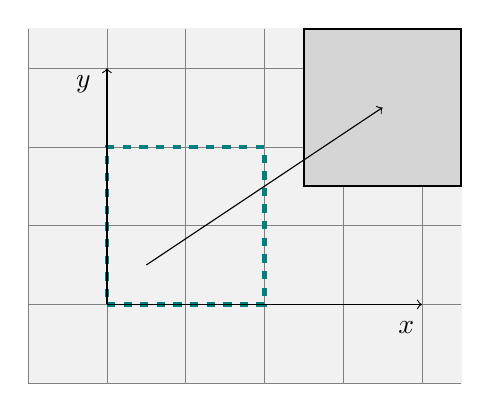
\begin{tikzpicture}
\draw[fill=gray!11,gray!11](0,0) rectangle (5.5,4.5);
\draw[step=1cm,gray,very thin] (0,0) grid (5.5,4.5); %background grid
\draw[ultra thick,dashed,teal] (1,1) -- (3,1) -- (3,3) -- (1,3) -- cycle;
\draw[thin,->]   (1,1) -- (5,1) ;
\draw[thin,->]   (1,1) -- (1,4) ;
\draw[fill=gray!33,thick] (3.5,2.5) -- (5.5,2.5) -- (5.5,4.5) -- (3.5,4.5) -- cycle; 
\node[] at (4.8,0.7) {$x$};
\node[] at (0.7,3.8) {$y$};
\draw[thin,->]   (1.5,1.5) -- (4.5,3.5) ;
\end{tikzpicture}
\end{center}


There is no deformation to speak of since the body remains the same but translated. The equation above also writes
\[
\left(
\begin{array}{c}
x \\ y
\end{array}
\right)
=
\underbrace{
\left(
\begin{array}{cc}
1 & 0 \\
0 & 1
\end{array}
\right)
}_{\bm F}
\cdot
\left(
\begin{array}{c}
X \\ Y
\end{array}
\right)
+
\left(
\begin{array}{c}
2.5 \\ 1.5
\end{array}
\right)
\]
We will see the significance of the matrix ${\bm F}$ in what follows.

\paragraph{Rigid body rotation} For instance:
\begin{eqnarray}
x &=& X \cos \theta - Y \sin \theta \\ 
y &=& X \sin \theta + Y \cos \theta 
\end{eqnarray}


\begin{center}
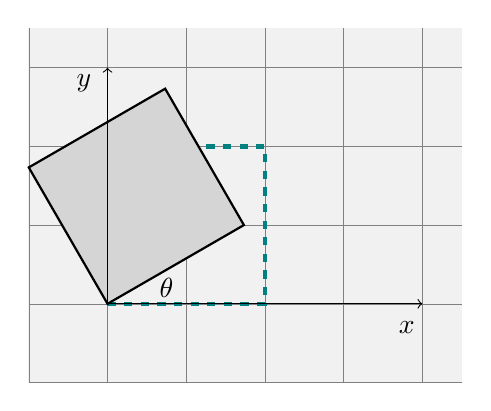
\begin{tikzpicture}
\draw[fill=gray!11,gray!11](0,0) rectangle (5.5,4.5);
\draw[step=1cm,gray,very thin] (0,0) grid (5.5,4.5); 
\draw[ultra thick,dashed,teal] (1,1) -- (3,1) -- (3,3) -- (1,3) -- cycle;
\draw[fill=gray!33,thick] (1,1) -- (2.732,2) -- (1.732,3.732) -- (0,2.732) -- cycle; 
\draw[thin,->]   (1,1) -- (5,1) ;
\draw[thin,->]   (1,1) -- (1,4) ;
\node[] at (4.8,0.7) {$x$};
\node[] at (0.7,3.8) {$y$};
\node[] at (1.75,1.2) {$\theta$};
\end{tikzpicture}
\end{center}



This can be rewritten as $\vec{x}={\bm F}\cdot \vec{X}$, where 
${\bm F}$ is a rotation matrix counter-clockwise about the $z$ axis (perpendicular
to the page):
\[
{\bm F} = 
\left(
\begin{array}{cc}
\cos\theta & -\sin\theta \\
\sin\theta & \cos\theta 
\end{array}
\right)
\]
Actually the body is not deformed, but simply rotated. There is no strain associated to this 
transformation. 


\paragraph{Stretching} Let us now turn to a 'real' deformation with shape change: stretching. 
For instance:

\begin{equation}
\begin{cases} 
x &=2X  \\ 
y &=1.5 Y 
\end{cases}
\qquad
\Leftrightarrow
\qquad
{\bm F} = 
\left(
\begin{array}{cc}
2 & 0 \\
0 & 1.5
\end{array}
\right)
\label{eq:stretching1}
\end{equation}

\begin{center}
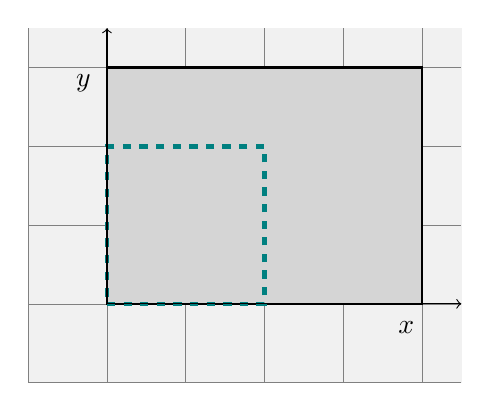
\begin{tikzpicture}
\draw[fill=gray!11,gray!11](0,0) rectangle (5.5,4.5);
\draw[step=1cm,gray,very thin] (0,0) grid (5.5,4.5); 
\draw[fill=gray!33,thick] (1,1) -- (5,1) -- (5,4) -- (1,4) -- cycle;
\draw[ultra thick,dashed,teal] (1,1) -- (3,1) -- (3,3) -- (1,3) -- cycle;
\draw[thin,->]   (1,1) -- (5.5,1) ;
\draw[thin,->]   (1,1) -- (1,4.5) ;
\node[] at (4.8,0.7) {$x$};
\node[] at (0.7,3.8) {$y$};
\end{tikzpicture}
\end{center}

This deformation has increased the area of the body by a factor 3.


\paragraph{Shearing} Another possible deformation (and a very relevant one 
in structural geology) is shearing:
\begin{equation}
\begin{cases} 
x &=X  \\ 
y &=\frac12 X + Y 
\end{cases}
\qquad
\Leftrightarrow
\qquad
{\bm F} = 
\left(
\begin{array}{cc}
1 & 0 \\
\frac12 & 1
\end{array}
\right)
\label{eq:shearing0}
\end{equation}



\begin{center}
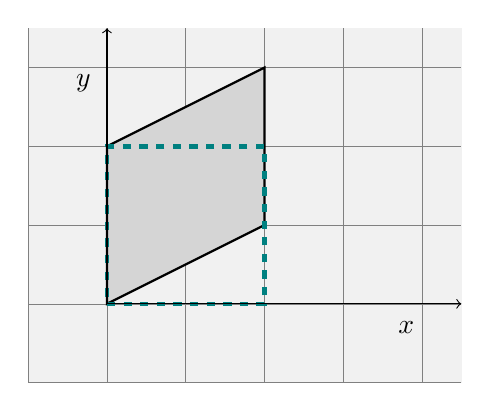
\begin{tikzpicture}
\draw[fill=gray!11,gray!11](0,0) rectangle (5.5,4.5);
\draw[step=1cm,gray,very thin] (0,0) grid (5.5,4.5); 
\draw[fill=gray!33,thick] (1,1) -- (3,2) -- (3,4) -- (1,3) -- cycle;
\draw[ultra thick,dashed,teal] (1,1) -- (3,1) -- (3,3) -- (1,3) -- cycle;
\draw[thin,->]   (1,1) -- (5.5,1) ;
\draw[thin,->]   (1,1) -- (1,4.5) ;
\node[] at (4.8,0.7) {$x$};
\node[] at (0.7,3.8) {$y$};
\end{tikzpicture}
\end{center}

This is a case of \underline{simple shear}: a deformation in which parallel planes in a material remain 
parallel and maintain a constant distance, while translating relative to each other. 
We see that the area of the body is conserved but not its shape.
\index{general}{Simple shear}


Let us now consider this shear example:

\begin{equation}
\begin{cases} 
x &=X + \frac12 Y \\ 
y &=\frac12 X + Y 
\end{cases}
\qquad
\Leftrightarrow
\qquad
{\bm F} = 
\left(
\begin{array}{cc}
1 & \frac12 \\
\frac12 & 1
\end{array}
\right)
\label{eq:shearing1}
\end{equation}

\begin{center}
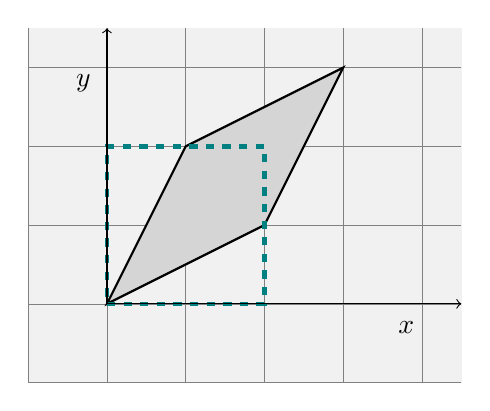
\begin{tikzpicture}
\draw[fill=gray!11,gray!11](0,0) rectangle (5.5,4.5);
\draw[step=1cm,gray,very thin] (0,0) grid (5.5,4.5); 
\draw[fill=gray!33,thick] (1,1) -- (3,2) -- (4,4) -- (2,3) -- cycle;
\draw[ultra thick,dashed,teal] (1,1) -- (3,1) -- (3,3) -- (1,3) -- cycle;
\draw[thin,->]   (1,1) -- (5.5,1) ;
\draw[thin,->]   (1,1) -- (1,4.5) ;
\node[] at (4.8,0.7) {$x$};
\node[] at (0.7,3.8) {$y$};
\end{tikzpicture}
\end{center}

Here too the shape changes and we obtain a parallelogram. However, 
the area is not conserved since the area of the undeformed square is 4, 
while the area of the parallelogram is 3
(Split it in two triangles. The area of the triangle inside the square is 4-1-1-0.5).

So while the expression for ${\bm F}$ above may superficially resemble 
pure shear (irrotational, area preserving shear), it is not. 
To describe pure shear with ${\bm F}$, the diagonal terms are no longer 1. 
The following shear example does describe pure shear:
\begin{equation}
\begin{cases} 
x &=1.25X + 0.75 Y \\ 
y &=0.75 X + 1.25Y 
\end{cases}
\qquad
\Leftrightarrow
\qquad
{\bm F} = 
\left(
\begin{array}{cc}
1.25 & 0.75 \\
0.75 & 1.25
\end{array}
\right)
=\frac14
\left(
\begin{array}{cc}
5 & 3 \\
3 & 5
\end{array}
\right)
\label{eq:shearing3}
\end{equation}

\begin{center}
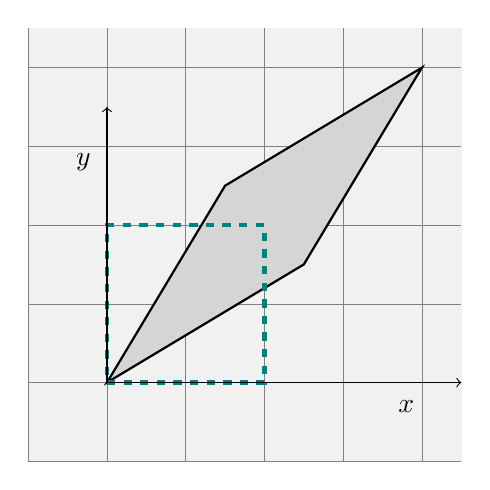
\begin{tikzpicture}
\draw[fill=gray!11,gray!11](0,0) rectangle (5.5,5.5);
\draw[step=1cm,gray,very thin] (0,0) grid (5.5,5.5); 
\draw[fill=gray!33,thick] (1,1) -- (3.5,2.5) -- (5,5) -- (2.5,3.5) -- cycle;
\draw[ultra thick,dashed,teal] (1,1) -- (3,1) -- (3,3) -- (1,3) -- cycle;
\draw[thin,->]   (1,1) -- (5.5,1) ;
\draw[thin,->]   (1,1) -- (1,4.5) ;
\node[] at (4.8,0.7) {$x$};
\node[] at (0.7,3.8) {$y$};
%\node[] at (1.75,1.2) {$\theta$};
\end{tikzpicture}
\end{center}

The area of the resulting parallelogram is still 1, so this deformation conserves volume.

 


%......................................................................
%\subsection*{Combination of deformations}

%So far we have then seen two types of deformation: stretching and shear, and these
%can also be accompanied by rotation. 
%It then makes sense to think of a deformed body as the result of successive 
%shearing, stretching and rotation. 


%\begin{center}
%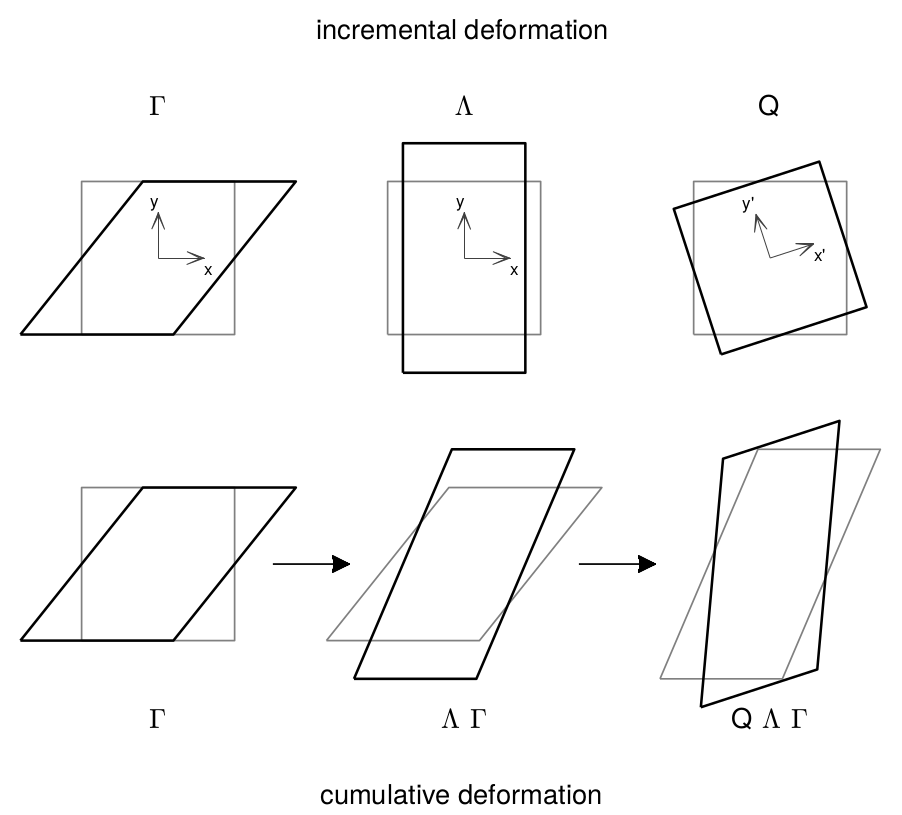
\includegraphics[width=8cm]{python_codes/fieldstone_89/images/broerse}\\
%{\captionfont Taken from Broerse et al, subm.
%Any homogeneous deformation ${\bm F}$ can be written as a succession of a simple shear
%parallel to x called ${\bm \Gamma}$; an extension in x and an extension in y direction called
%${\bm \Lambda}$; followed by an orthogonal rotation ${\bm Q}$. 
%Here, the change between initial line vectors $d\vec{X}$ (in this case
%the side vectors of a square) to final initial line vectors $d\vec{x}$ (the deformed quadrilaterals) is
%determined by: $d\vec{x} = {\bm F} \cdot d\vec{X}$. 
%First row, incremental deformation, second row, cumulative deformation.
%}
%\end{center}


%Thinking of ${\bm F}$ as the matrix which transforms $\vec{X}$ into $\vec{x}$
%it then makes sense to decompose it into the product of three matrices, 
%one accounting for rotation ${\bm R}$ (or ${\bm Q}$ as in the example above), 
%one for stretching ${\bm \Lambda}$ and
%one for shearing ${\bm \Gamma}$.
%However, there is a caveat in this approach: it is easy to show that 
%these transformations do not necessarily commute, i.e. the order in which 
%these transformations are succesively applied matters.

%We then write
%\[
%{\bm F} = {\bm R} \cdot {\bm \Lambda} \cdot {\bm \Gamma}
%\] 

%......................................................................
\subsection*{Polar decomposition of ${\bm F}$}

A polar decomposition separates ${\bm F}$ into a rotation and a stretching of 
the space along a set of orthogonal axes\footnote{\url{https://en.wikipedia.org/wiki/Polar_decomposition}}. 
\index{general}{Polar Decomposition}

For instance, let us now consider the following transformation:
\begin{equation}
\begin{cases} 
x &= 1.3X-0.375Y\\ 
y &= 0.75X+0.65 Y
\end{cases}
\qquad
\Leftrightarrow
\qquad
{\bm F} = 
\left(
\begin{array}{cc}
1.3 & -0.375 \\
0.75 & 0.650
\end{array}
\right)
\end{equation}
It can be decomposed as 
\[
{\bm F} = {\bm R} \cdot {\bm U}
=
\left(
\begin{array}{cc}
0.866 & -0.5 \\
0.5 & 0.866
\end{array}
\right)
\cdot
\left(
\begin{array}{cc}
1.5 & 0 \\
0 & 0.75
\end{array}
\right)
\]
where ${\bm R}$ is the aforementioned rotation,  
${\bm U}$ is the right stretch tensor, or as \index{general}{Right stretch Tensor} 
\[
{\bm F} = {\bm V} \cdot {\bm R}
=
\left(
\begin{array}{cc}
1.313 & 0.325 \\
0.325 & 0.938 
\end{array}
\right)
\cdot
\left(
\begin{array}{cc}
0.866 & -0.5 \\
0.5 & 0.866
\end{array}
\right)
\]
where ${\bm V}$ is the left stretch tensor. \index{general}{Left stretch Tensor} 
We see that ${\bm U}\ne {\bm V}$ but it can 
easily be proven that 
\[
{\bm V} = {\bm R}\cdot{\bm U}\cdot {\bm R}^T
\qquad
\text{and}
\qquad
{\bm U} = {\bm R}^T\cdot{\bm V}\cdot {\bm R}
\]
Note that  ${\bm V}$ and ${\bm U}$ are symmetric, and have positive eigenvalues, and the 
eigenvalues correspond to stretches in $[0,\infty]$.
These stretches then form the axes of a strain ellipse. 
$U$ and $V$ have furthermore the same eigenvalues, but their eigenvectors are 
rotated with regards to each other since ${\bm U} = {\bm R}^T \cdot {\bm V} \cdot {\bm R}$ (which is basically a coordinate rotation).



\begin{center}
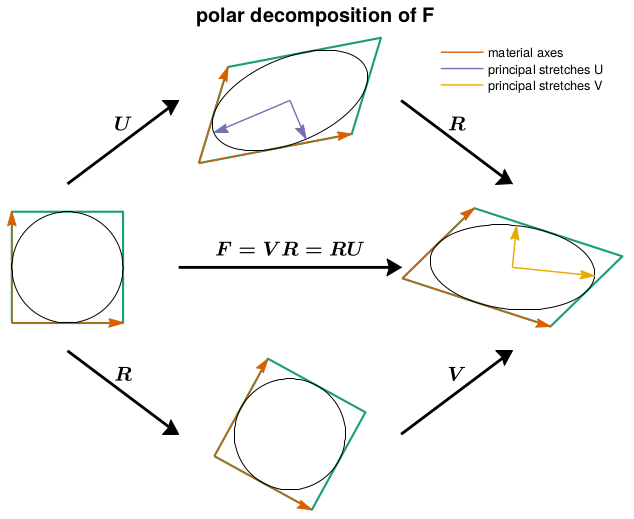
\includegraphics[width=8cm]{python_codes/fieldstone_89/images/polardec}\\
{\captionfont Taken from Broerse et al, subm. 
Sketch of the polar decomposition of the deformation gradient ${\bm F}$ into an orthogonal
rotation $R$ and symmetric stretch tensors $V$ or $U$. Here we apply the deformation of $F$ to an
initially square material element, with side vectors $d\vec{X}$. 
The deformed configuration (right)
leads to an element with side vectors $dx = FdX$. 
The decomposition can be written as first
a stretch $U$ followed by a rotation $R$, or first a rotation $R$ followed by a stretch $V$. 
Principal stretches $\vec\lambda$ of $V$ provide the stretch in the final, deformed, configuration, 
whereas stretches $\vec\lambda$ of $U$ provide the stretch in the original configuration. 
Material axes provide reference for the reader. 
We also show strain ellipses in black, that can be constructed using circle coordinates
as $dX$. Because $V$ and $U$ are symmetric tensors, the rotation angle of $R$ is non-zero for simple
shear contributions.}
\end{center}





\begin{itemize}
\item
The actual decomposition algorithm is not trivial, 
even for $2\times2$ matrices. This is nicely documented 
online\footnote{\url{http://www.continuummechanics.org/polardecomposition.html}}.
For instance, coming back to the simple shear example of Eq.~\eqref{eq:shearing0}, 
the tensor ${\bm F}$ can be written 
\[
{\bm F}= {\bm R} \cdot {\bm U}
=
\left(
\begin{array}{cc}
\cos\theta & -\sin\theta \\
\sin\theta & \cos\theta 
\end{array}
\right)
\cdot
\left(
\begin{array}{cc}
U_{xx} & U_{xy} \\
U_{yx} & U_{yy} 
\end{array}
\right)
\]
We must then determine $U_{ij}$ and $\theta$ which is, once again, not trivial. We then use the method 
of Hoger \& Carlson(1984) \cite{hoca84} (see note in a couple of pages further). We start by computing
\[
{\bm C} =
 {\bm F}^T\cdot{\bm F}
=
\left(
\begin{array}{cc}
1 & 1/2 \\ 
0 & 1
\end{array}
\right)
\cdot
\left(
\begin{array}{cc}
1 & 0 \\ 
1/2 & 1
\end{array}
\right)
=
\left(
\begin{array}{cc}
5/4 & 1/2 \\ 
1/2 & 1
\end{array}
\right)
\]
We then proceed by computing the 1st and 2nd invariants of ${\bm C}$:
\begin{eqnarray}
I_C &=&C_{xx}+C_{yy}=5/4+1=9/4 \nonumber\\
II_C&=&C_{xx}C_{yy}-C_{xy}C_{yx} = 5/4-1/4 = 1 \nonumber
\end{eqnarray}
and of ${\bm U}$
\begin{eqnarray}
I_U &=&\sqrt{I_C + 2 \sqrt{II_C}} = \sqrt{9/4 + 2 }= \frac{1}{2}\sqrt{17} \nonumber\\
II_U&=&\sqrt{II_C} = 1 \nonumber
\end{eqnarray}
Then the right stretch tensor is:
\[
{\bm U} = \frac{1}{I_U}({\bm C} + II_U {\bm I})
=
\frac{2}{\sqrt{17}}  \left[ 
\left(
\begin{array}{cc}
5/4 & 1/2 \\ 
1/2 & 1
\end{array}
\right)
+ 
\left(
\begin{array}{cc}
1 &0 \\ 0 & 1
\end{array}
\right)
\right]
=
\frac{2}{\sqrt{17}}  
\left(
\begin{array}{cc}
9/4 & 1/2 \\ 
1/2 & 2
\end{array}
\right)
\]
The inverse is simply:
\[
{\bm U}^{-1} 
=\frac{1}{U_{xx}U_{yy}-U_{xy}U_{yx}}
\left(
\begin{array}{cc}
U_{yy} & -U_{xy} \\
-U_{yx} & U_{xx} 
\end{array}
\right)
=
\frac{2}{\sqrt{17}}
\left(
\begin{array}{cc}
2 & -1/2 \\
-1/2 & 9/4
\end{array}
\right)
\]
Finally 
\[
{\bm R} = {\bm F} \cdot {\bm U}^{-1}
=
\left(
\begin{array}{cc}
1 & 0 \\
\frac12 & 1
\end{array}
\right)
\cdot
\frac{2}{\sqrt{17}}
\left(
\begin{array}{cc}
2 & -1/2 \\
-1/2 & 9/4
\end{array}
\right)
=
\frac{2}{\sqrt{17}}
\left(
\begin{array}{cc}
2 & -1/2 \\
1/2 & 2
\end{array}
\right)
\]
Finally 
\[
\theta = \arctan R_{yx}/R_{xx} = \arctan \frac14 \simeq 14^o
\]
This is very important since it means that simple shear deformation generates rotation! 

It is also worth noting that since $\theta=14^o$, then the rotation matrix is 
\[
{\bm R} 
=
\left(
\begin{array}{cc}
\cos\theta & -\sin\theta \\
\sin\theta & \cos\theta 
\end{array}
\right)
\simeq
\left(
\begin{array}{cc}
0.9701 &  -0.2425 \\
0.2425 & 0.9701 
\end{array}
\right)
\simeq
{\bm I} + 
\left(
\begin{array}{cc}
0 &  -0.2425 \\
0.2425 & 0 
\end{array}
\right)
\]


\item
Looking now at Eq.~\eqref{eq:shearing3}, then
\[
{\bm C} = {\bm F}^T\cdot{\bm F}
=
\frac{1}{8}
\left(
\begin{array}{cc}
17 & 15 \\
15 & 17
\end{array}
\right)
\]
We then proceed by computing the 1st and 2nd invariants of ${\bm C}$:
\begin{eqnarray}
I_C &=&C_{xx}+C_{yy} = 17/4\\
II_C&=&C_{xx}C_{yy}-C_{xy}C_{yx} = (17^2-15^2)/64 = 1
\end{eqnarray}
and of ${\bm U}$
\begin{eqnarray}
I_U &=&\sqrt{I_C + 2 \sqrt{II_C}} = \sqrt{ 17/4 + \sqrt{1}  } = \frac{5}{2}\\
II_U&=&\sqrt{II_C} = 1
\end{eqnarray}
Then the right stretch tensor is:
\[
{\bm U} = \frac{1}{I_U}({\bm C} + II_U {\bm I})
=
\frac{2}{5}
\frac{1}{8}
\left(
\begin{array}{cc}
17+8 & 15 \\
15 & 17+8
\end{array}
\right)
=
\frac{1}{4}
\left(
\begin{array}{cc}
5 & 3 \\
3 & 5
\end{array}
\right)
\]
Its inverse is 
\[
{\bm U}^{-1}
=
\frac{1}{4}
\left(
\begin{array}{cc}
5 & -3 \\
-3 & 5
\end{array}
\right)
\]
and finally 
\[
{\bm R}= {\bm F} \cdot {\bm U}^{-1}
=
\frac{1}{4}
\left(
\begin{array}{cc}
5 & 3 \\
3 & 5
\end{array}
\right)
\cdot
\frac{1}{4}
\left(
\begin{array}{cc}
5 & -3 \\
-3 & 5
\end{array}
\right)
={\bm I}
\]
This corresponds to an angle $\theta=0^o$, i.e. it is an irrotational deformation, and since
we have shown that it conserves volume, it is \underline{pure shear}.

Pure shear is an example of irrotational strain in which body is elongated in one direction 
while being shortened perpendicularly. Indeed, in this case we have extended the body 
along the (1,1) direction while squeezing it in the orthogonal (1,-1) direction.
Pure shear is differentiated from simple shear in that pure shear involves no rigid body rotation. 
\index{general}{Pure Shear}

\end{itemize}


\newpage
%%%%%%%%%%%%%%%%%%%%%%%%%%%%%%%%%%%%%%%%%%%%%%%%%%%%%%%%%%%%%%%%%%%%%%5
\subsection*{The deformation gradient}

There remains to formally define ${\bm F}$ as the deformation gradient.
\index{general}{Deformation Gradient}
It is defined as :
\[
\boxed{
{\bm F} = (\vec\nabla_X \vec{x})^T
= 
\left(\frac{\partial \vec{x}}{\partial \vec{X}} \right)^T
=
\left(
\begin{array}{cc}
\frac{\partial x}{\partial X} & 
\frac{\partial y}{\partial X} \\ \\
\frac{\partial x}{\partial Y} & 
\frac{\partial x}{\partial Y}  
\end{array}
\right)^T
=
\left(
\begin{array}{cc}
\frac{\partial x}{\partial X} & 
\frac{\partial x}{\partial Y} \\ \\
\frac{\partial y}{\partial X} & 
\frac{\partial x}{\partial Y}  
\end{array}
\right)
}
\]
The transpose is necessary and best explained through example. 
Looking at the first shearing example of Eq.~\eqref{eq:shearing1} again, we have

\begin{equation}
\begin{cases} 
x &=X  \\ 
y &=\frac12 X + Y 
\end{cases}
\qquad
\Leftrightarrow
\qquad
{\bm F} = 
\left(
\begin{array}{cc}
1 & 0 \\
\frac12 & 1
\end{array}
\right)
\label{eq:shearing2}
\end{equation}
and 
\[
\vec\nabla_{X}  \vec{x}=
\left(
\begin{array}{cc}
\frac{\partial x}{\partial X} & 
\frac{\partial y}{\partial X} \\ \\
\frac{\partial x}{\partial Y} & 
\frac{\partial x}{\partial Y}  
\end{array}
\right)
=
\left(
\begin{array}{cc}
1 & \frac12 \\ 
0 & 1
\end{array}
\right)
\]
which is indeed the transpose of ${\bm F}$.


We can write the displacement $\vec{u}$ as the difference between current and reference coordinates:
\[
\vec{u} = \vec{x}-\vec{X}
\]
and the deformation gradient can be reformulated as a function of the displacements:
\[
{\bm F} 
= \frac{\partial \vec{x}}{\partial \vec{X}} 
= \frac{\partial }{\partial \vec{X}} (\vec{X}+\vec{u})
= {\bm I} + \frac{\partial \vec{u}}{\partial \vec{X}} 
= {\bm I} + \vec{\nabla}\vec{u} 
\]
From this it follows that the infinitesimal strain tensor can be written
\[
\boxed{
{\bm \varepsilon}(\vec{u}) = \frac{1}{2}( \vec\nabla\vec{u} + \vec\nabla\vec{u}^T )
= \frac{1}{2} (  {\bm F} +  {\bm F}^T) - {\bm I} 
}
\]
and the rotation tensor is then 
\[
{\bm \omega} 
=\frac{1}{2}( \vec\nabla\vec{u} - \vec\nabla\vec{u}^T )
= \frac{1}{2} (  {\bm F} -  {\bm F}^T)
\]

\index{general}{Infinitesimal Strain Tensor}


%-------------------------------------------------------------
\subsection*{Purpose of this stone}

This stone has two purposes:
\begin{itemize}
\item put the theory above into practice 
\item show that the 'standard' way of integrating strain on Lagrangian markers in 
geodynamical codes is merely an approximation and that this approximation 
no longer holds for large deformations/rotations. In other words, 
integrated strain rates lose their physical meaning when 
the deformation becomes large!
\end{itemize}

In all what follows we denote by 'old' the method by which 
strain is accumulated onto markers by time integration of the strain rate components.
In practice here we interpolate $\vec\nabla \vec\upnu $ through $Q_1$ shape functions
in the middle of the Lagrangian grid cells, we compute $\dot{\varepsilon}_{ij}$, we
update the strain as $\varepsilon_{ij} += \dot{\varepsilon}_{ij} \delta t$.
As we will show, this is fine only for (very) small total strains. 

The 'new' method computes the marker strain by means 
of the deformation tensor.
For each cell centroid, we compute the displacement gradient tensor ${\bm F}$, 
then carry out polar decomposition to write ${\bm F}$ as product of stretch and rotation, 
i.e. ${\bm F}=  {\bm V}\cdot {\bm R}$.
From ${\bm V}$ we compute the principal stretches $\lambda_{1,2}$ (eigenvalues of ${\bm V}$) 
and the eigenvectors as well since these represent the axes of the strain ellipse, 
i.e. the directions of maximum stretch.
We then substract 1 to principal stretches to get principal strains, $\varepsilon_{1,2} = \lambda_{1,2}-1$.

The 'new' method (which is not that new since it is to be found in Malvern (1969) \cite{malvern} 
is as accurate as the measurement of ${\bm F}$ itself, and the difference tells us how bad 
the 'old' method actually can be (spoiler alert: up to few tens of \%).


%MOVE elsewhere:
%Also principal strains can never be smaller than -1 by def, because less than -1 means
%more than 100\%  shortening (in 1D). but no upper limit.
%conversely principal stretch > 0 (bc it is strain +1 ).


 

\newpage
%------------------------------------------------------------------------
\subsection*{Polar decomposition a la Hoger \& Carlson (1984)}

The polar decomposition of ${\bm F}$ is not trivial, but an 
application of the Cayley-Hamilton theorem allows for this 
as explained in Hoger \& Carlson (1984) \cite{hoca84}.

The deformation gradient tensor ${\bm F}$ is computed in the middle of
each cell at a given time $t$ as follows:
\[
{\bm F}(t)
=
\left(
\begin{array}{cc}
F_{xx} & F_{xy} \\
F_{yx} & F_{yy} 
\end{array}
\right)
=
{\bm I}+
\left(
\begin{array}{cc}
\frac{\partial (x(t)-x_0)}{\partial x}  & \frac{\partial (x(t)-x_0)}{\partial y}  \\
\frac{\partial (y(t)-y_0)}{\partial x}  & \frac{\partial (y(t)-y_0)}{\partial y}  
\end{array}
\right)
\]
In what follows we omit the time dependence '$(t)$'.
Each cell is assumed to be a $Q_1$ quadrilateral with a marker at each corner. We therefore store the 
initial position of markers, and make use of bilinear $Q_1$ shape functions to compute the derivatives
above in the center of the cell.

\begin{enumerate}
\item The right Cauchy-Green deformation tensor is defined as
\[
{\bm C} = {\bm F}^T {\bm F}
= ({\bm R}\cdot {\bm U})^T \cdot ({\bm R} \cdot {\bm U})
= {\bm U}^T \cdot {\bm R}^T \cdot {\bm R} \cdot {\bm U}
= {\bm U}^T \cdot {\bm U}
\]
\item 
We then find the eigenvalues of ${\bm C}$:
\[
\mu_{1,2} = \frac{1}{2}(C_{xx}+C_{yy}) \pm \sqrt{ \frac{1}{4}(C_{xx}-C_{yy})^2 + C_{xy}^2   }
\]
\item We compute the two invariants:
\[
I_C = \mu_1+\mu_2 \qquad II_C = \mu_1\mu_2 
\]
\item Compute invariants of right stretch tensor U
\[
I_U=\sqrt{I_C+2\sqrt{II_C}}
\qquad
II_U=\sqrt{II_C}
\]
\item compute right stretch tensor ${\bm U}$
\[
{\bm U} = \frac{{\bm C}+ II_U {\bm I}}{I_U}
\]
\item compute inverse of ${\bm U}$
\[
{\bm U}^{-1} = - I_U \frac{{\bm C}- (II_U+I_C){\bm I}}{II_U(II_U+I_C)+II_C}
\]
\item compute rotation matrix ${\bm R}={\bm F}{\bm U}^{-1}$

\item compute left stretch tensor ${\bm V}={\bm F}{\bm R}^T$

\item Compute eigenvalues of ${\bm V}$, which are the square roots of those of ${\bm C}$
\[
\lambda_1 = \sqrt{\mu_1}
\qquad
\lambda_2 = \sqrt{\mu_2}
\]

\end{enumerate}










\newpage
%%%%%%%%%%%%%%%%%%%%%%%%%%%%%%%%%%%%%%%%%%%%%%%%%%%%%%%%%%%%%%%%%%%%%%5
\subsection*{The shear band (experiment=1)}

The domain is a rectangle of size $L_x\times L_y$ discretised by nelx $\times$ nely $Q_2$ elements.
The following velocity field is precribed in the domain:
\begin{eqnarray}
u(x,y)&=&0 \\
v(x,y)&=&\text{erf} [A(x-L_x/2)]
\end{eqnarray}

A swarm of $41\times41$ markers is then placed in the domain, 
and they are then painted as shown here:
\begin{center}
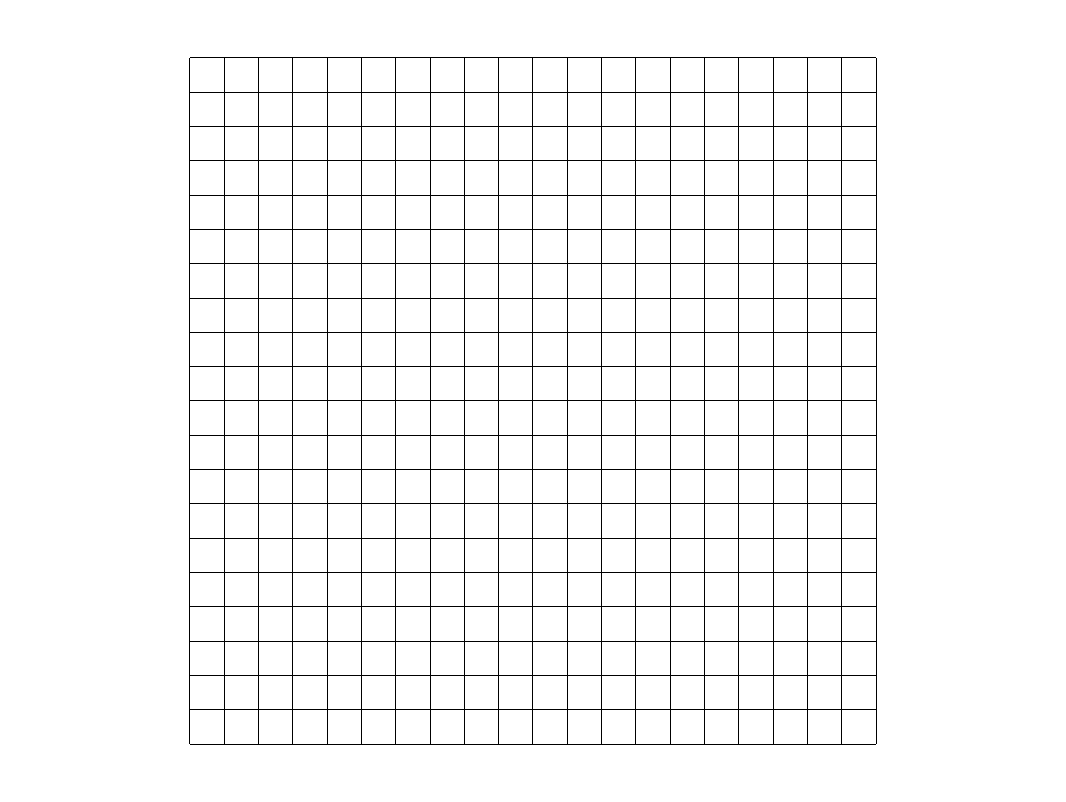
\includegraphics[width=5.6cm]{python_codes/fieldstone_89/results/shearband/init/grid}
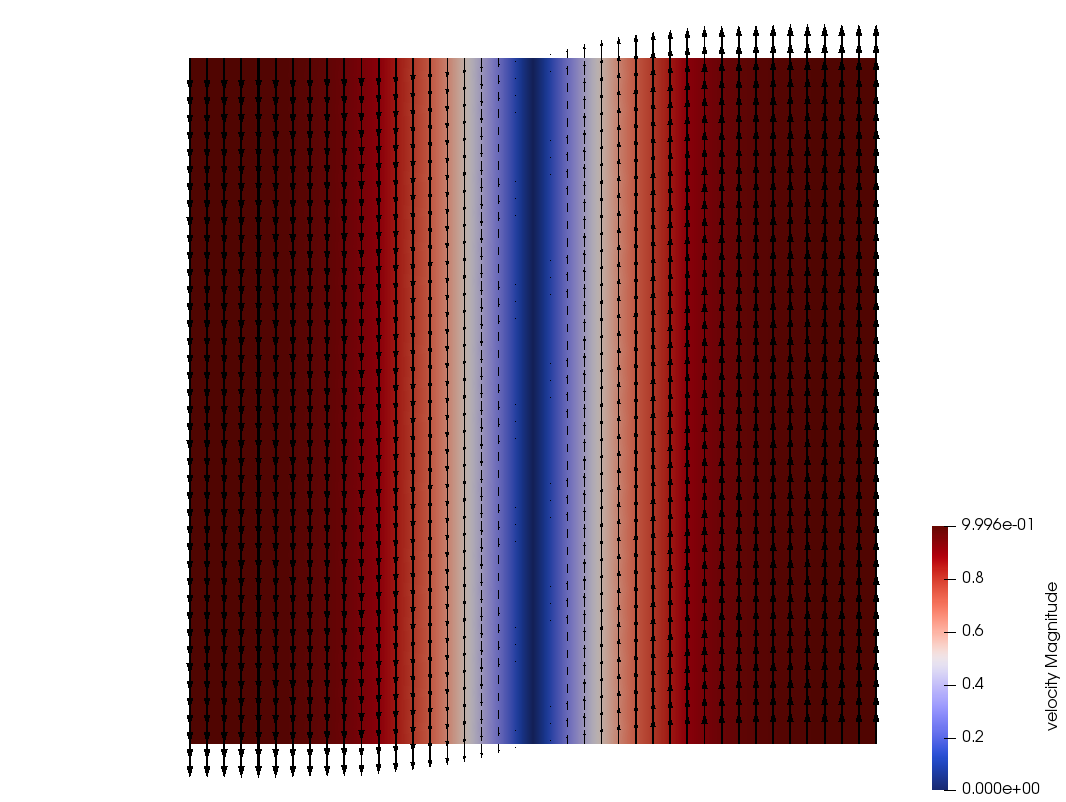
\includegraphics[width=5.6cm]{python_codes/fieldstone_89/results/shearband/init/vel}
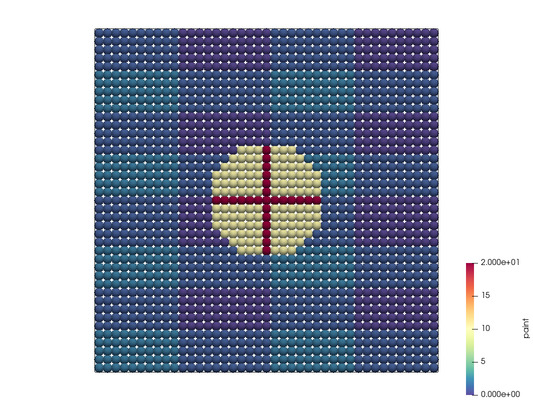
\includegraphics[width=5.6cm]{python_codes/fieldstone_89/results/shearband/init/markers}\\
{\captionfont Domain is unit square, resolution $20\times20$ elements. $A=5$. 
Left: Eulerian grid; Middle: velocity field; Right: marker initial position.}
\end{center}

A time loop is implemented. At each time step the velocity field of the grid is 
interpolated onto each marker that is in turn advected with a simple euler step. 
\[
\vec{x}(t+\delta t) = \vec{x}(t) + \vec\upnu \; \delta t
\]
Note that the timestep value $\delta t$ is controlled by means of a CFL condition 
with ${\cal C}=0.1$. Likewise, the components of the strain rate tensor are computed on each marker and 
used to update the strain on each marker:
\[
\varepsilon_{ij}(t+\delta t) = \varepsilon_{ij}(t) + \dot\varepsilon_{ij}(t) \; \delta t
\]
These markers form a Lagrangian mesh which deforms over time:
\begin{center}
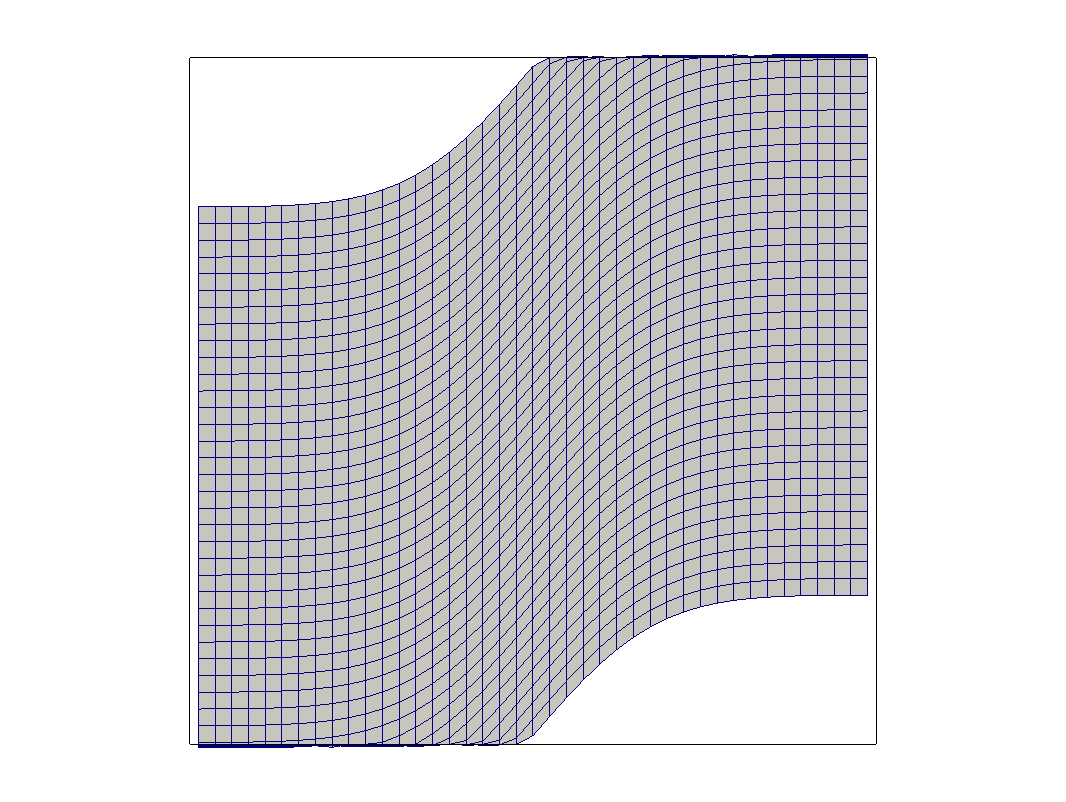
\includegraphics[width=6cm]{python_codes/fieldstone_89/results/shearband/init/swarm_mesh}
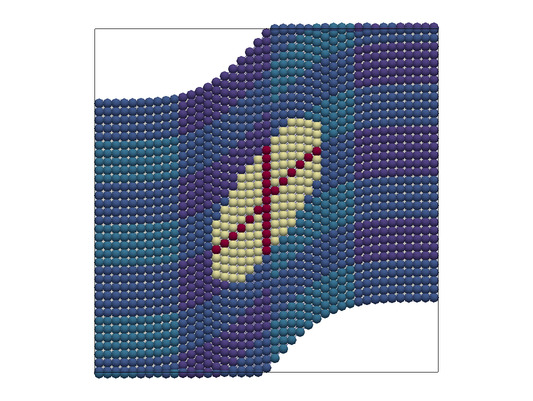
\includegraphics[width=6cm]{python_codes/fieldstone_89/results/shearband/init/swarm_paint}\\
{\captionfont Lagrangian mesh after 50 time steps.}
\end{center}
Markers which are advected outside of the domain are simply flagged inactive and these
are no longer advected. If one marker of a cell is flagged inactive so is the cell itself. 

At each time step the cumulative strain $\varepsilon_{ij}$ components are
computed at the center of the marker cells, as well as the principal strains $\varepsilon_1$ 
and $\varepsilon_2$ and the direction $\theta_\varepsilon$ of the principal strain:

\begin{center}
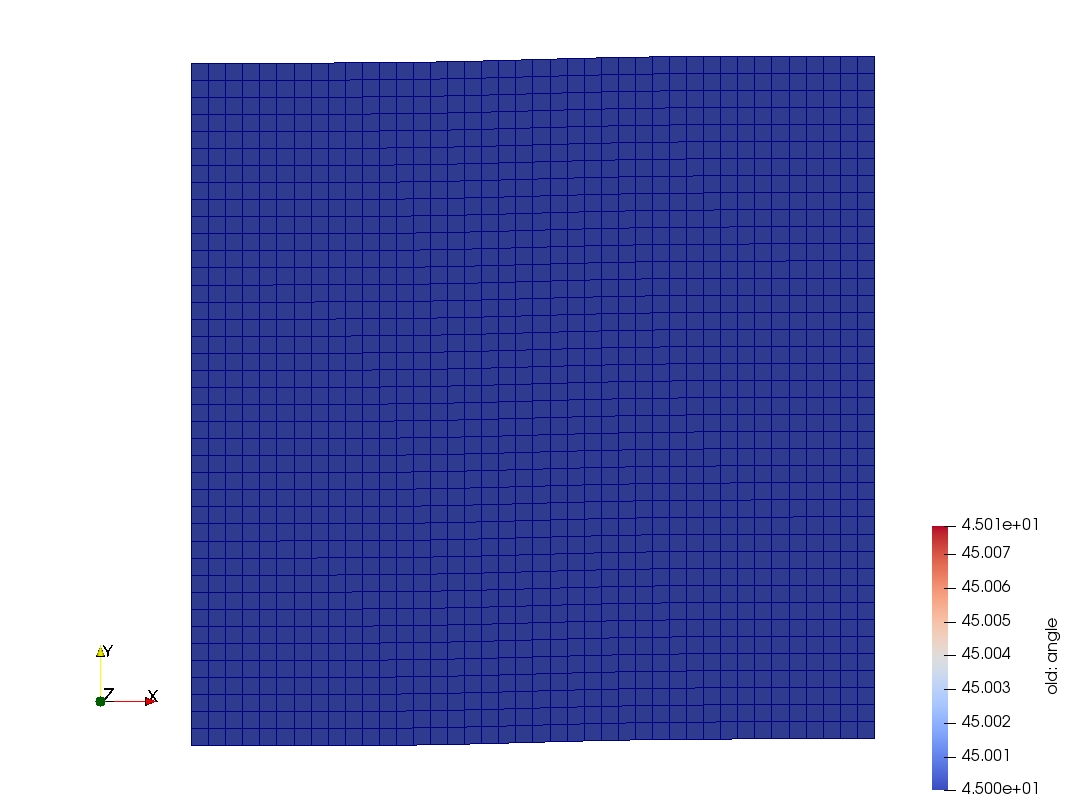
\includegraphics[width=6cm]{python_codes/fieldstone_89/results/shearband/old_angle_00}
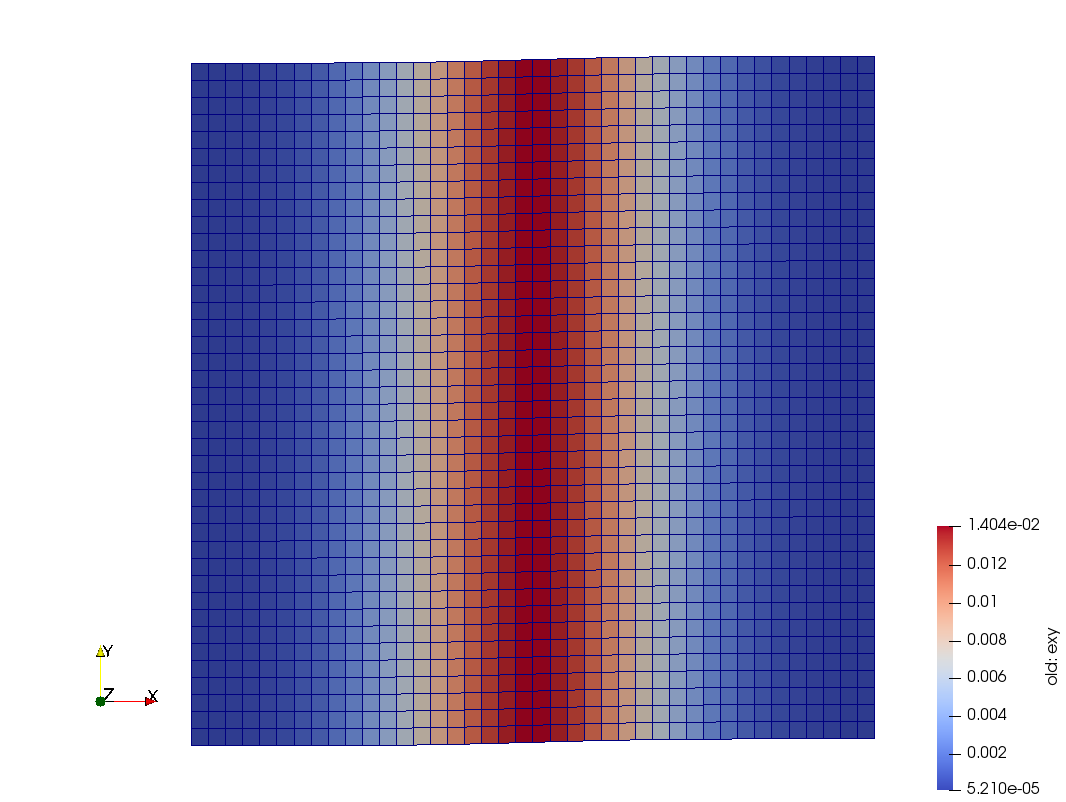
\includegraphics[width=6cm]{python_codes/fieldstone_89/results/shearband/old_exy_00}\\
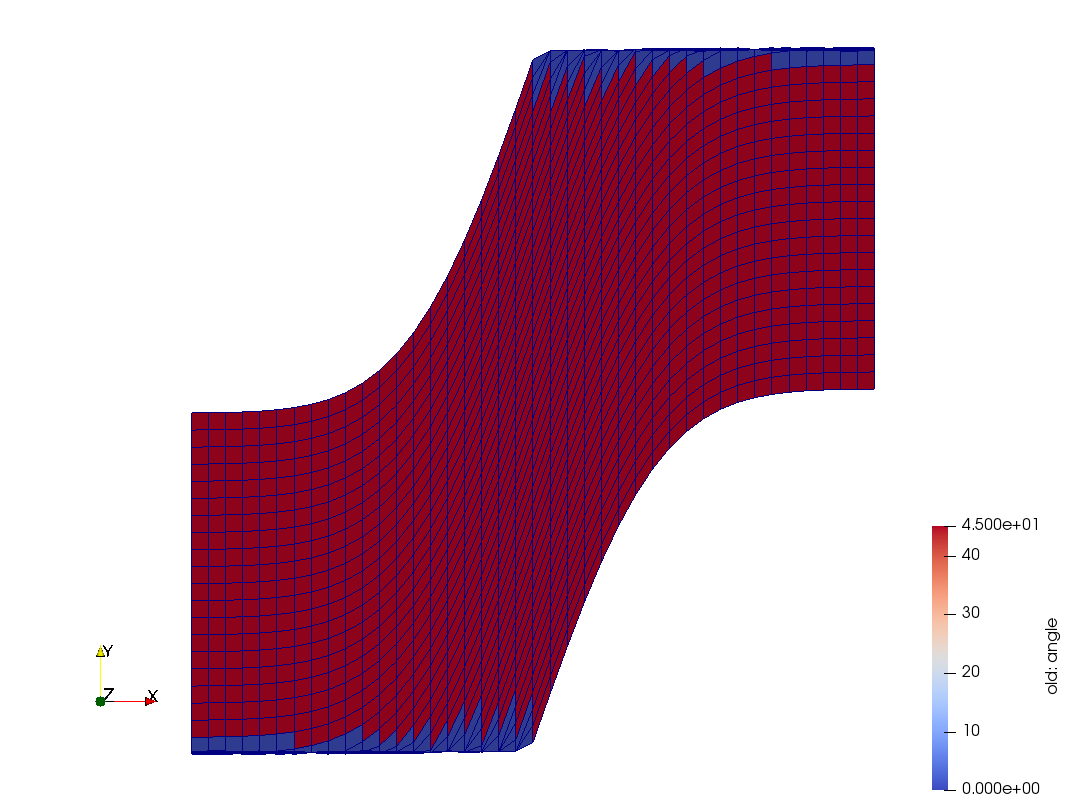
\includegraphics[width=6cm]{python_codes/fieldstone_89/results/shearband/old_angle_100}
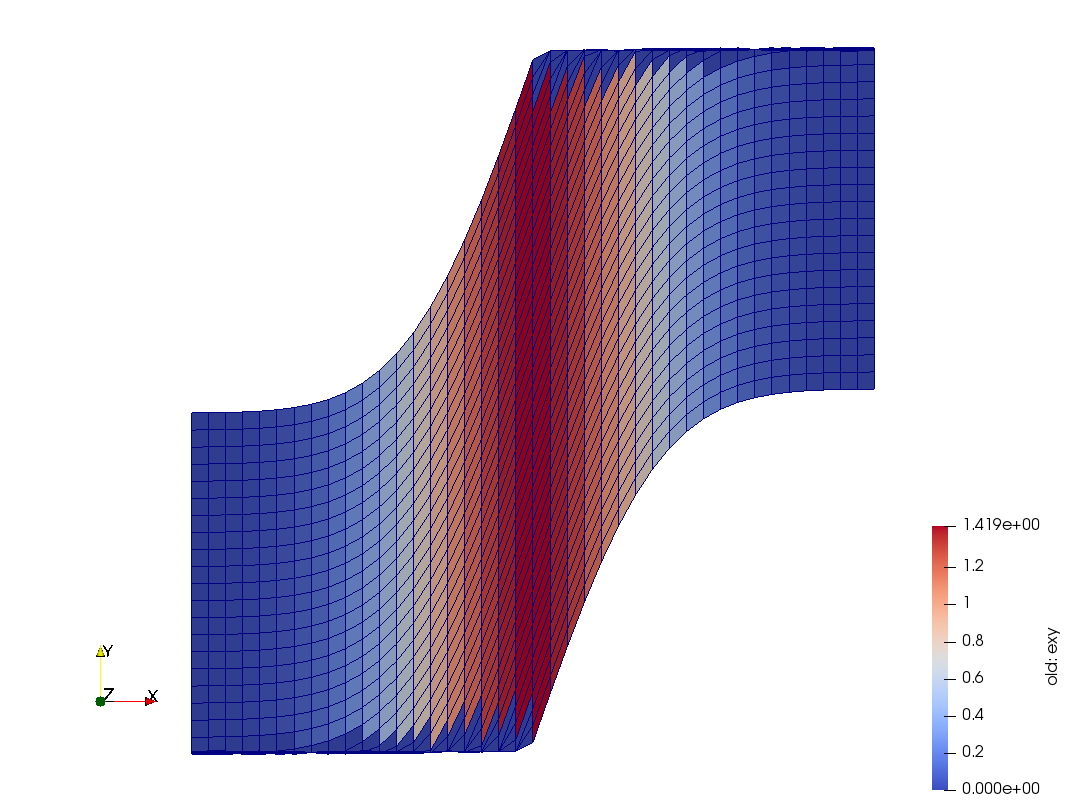
\includegraphics[width=6cm]{python_codes/fieldstone_89/results/shearband/old_exy_100}\\
{\captionfont Left: principal strain directions, Right: $\varepsilon_{xy}$.
Top row: first time step; Bottom row: 100th time step.}
\end{center}


\begin{center}
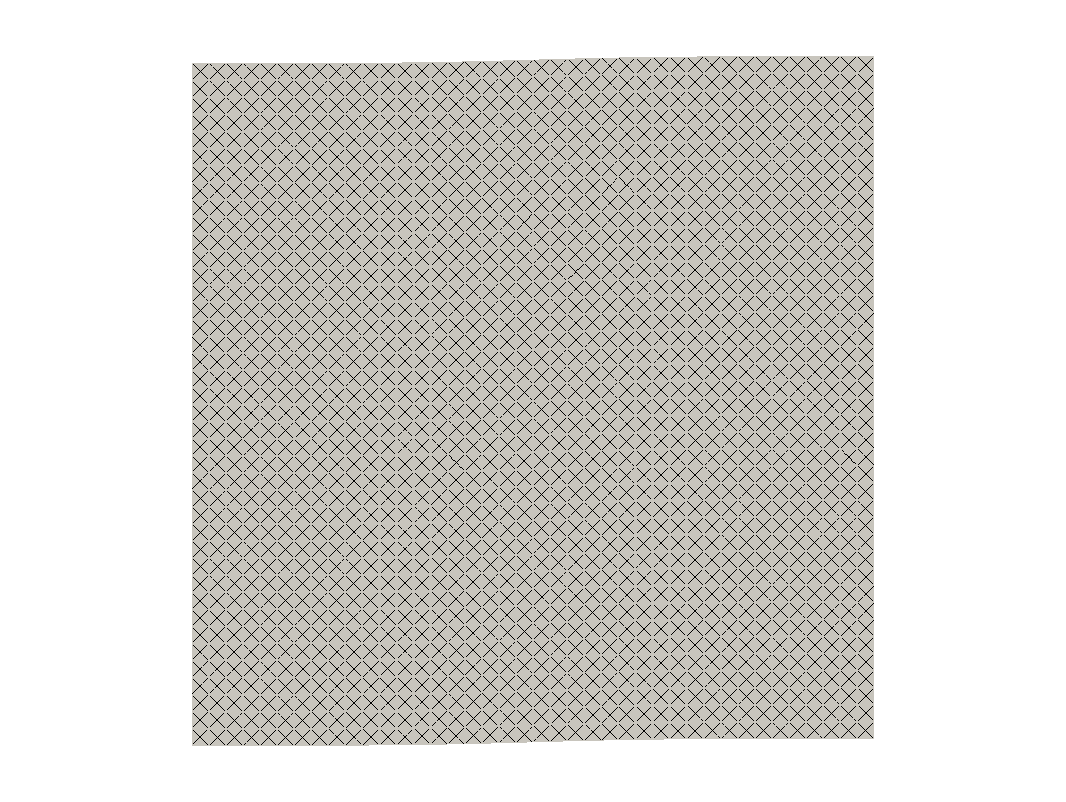
\includegraphics[width=5cm]{python_codes/fieldstone_89/results/shearband/old_dirs0000}
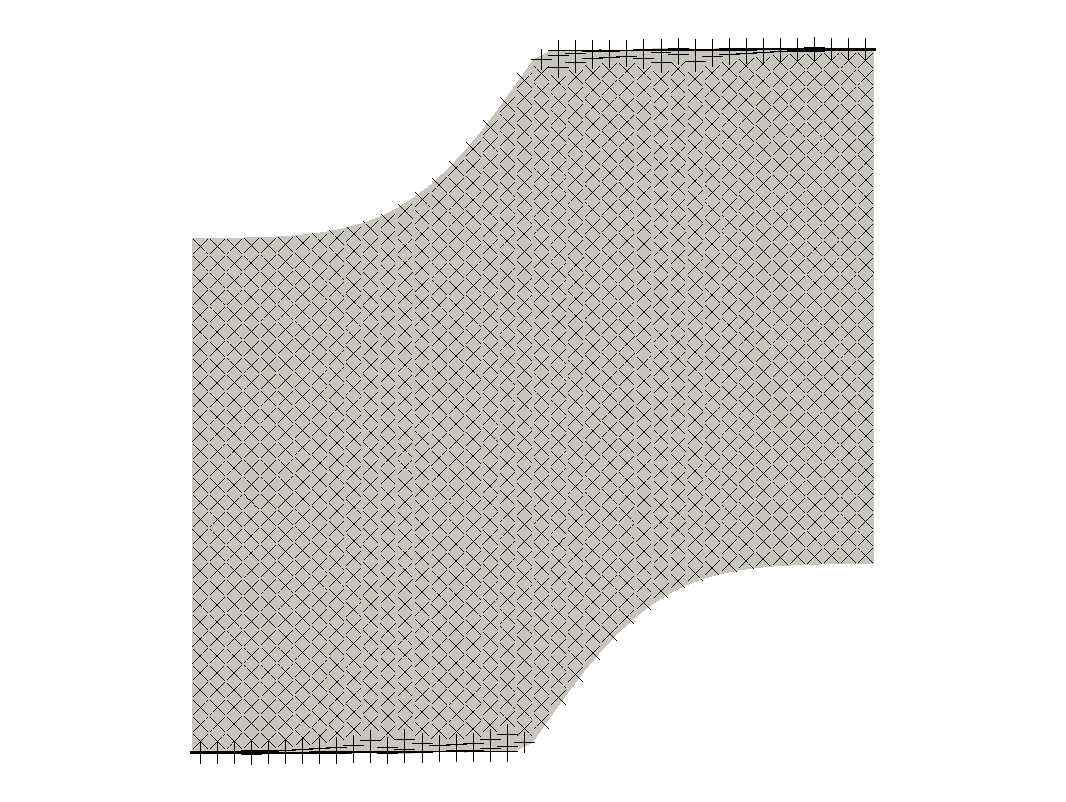
\includegraphics[width=5cm]{python_codes/fieldstone_89/results/shearband/old_dirs0005}
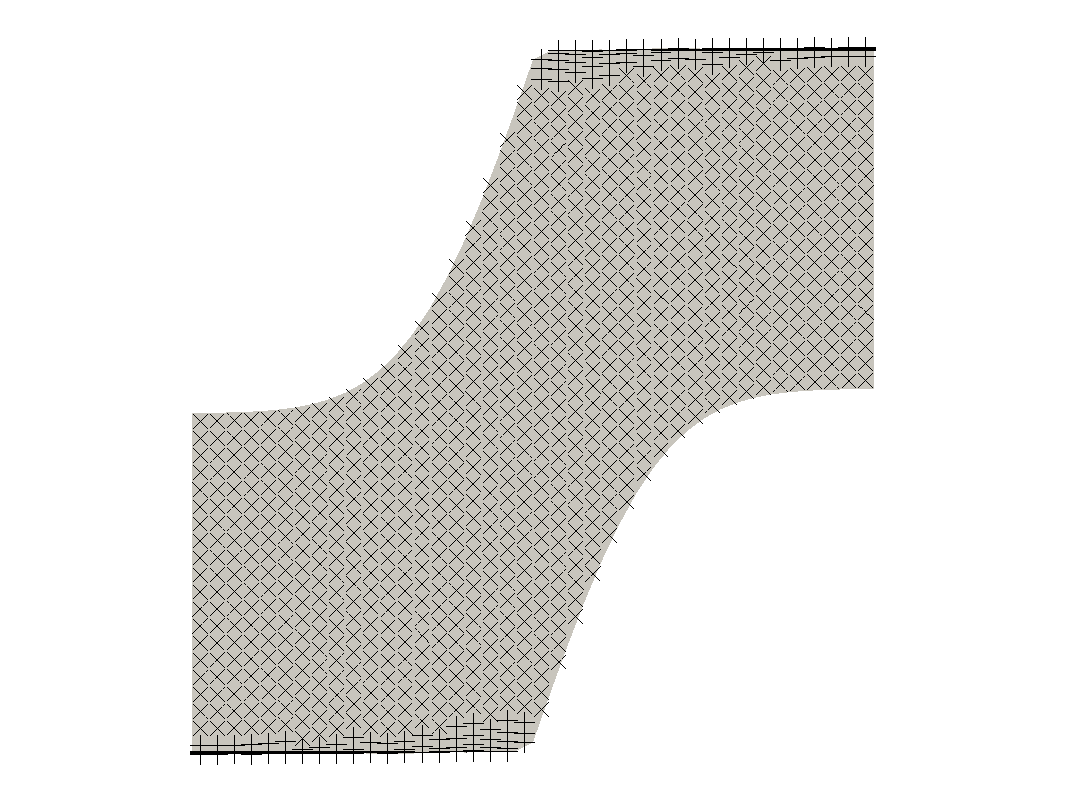
\includegraphics[width=5cm]{python_codes/fieldstone_89/results/shearband/old_dirs0010}\\
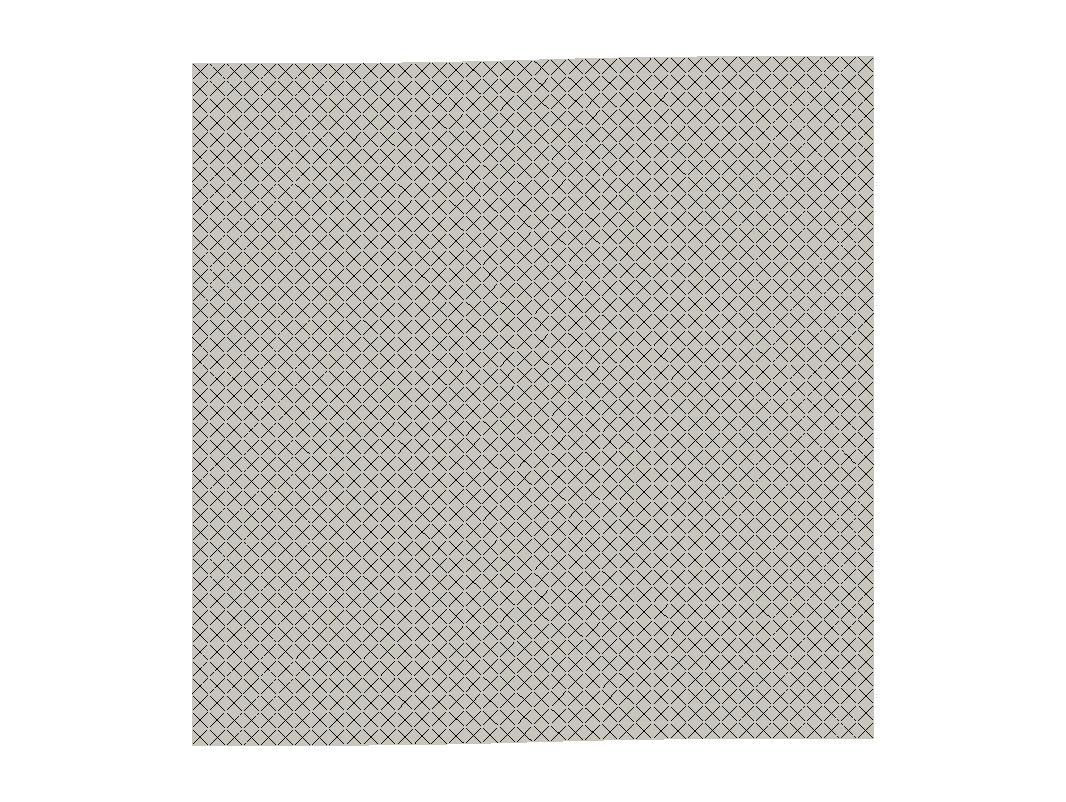
\includegraphics[width=5cm]{python_codes/fieldstone_89/results/shearband/new_dirs0000}
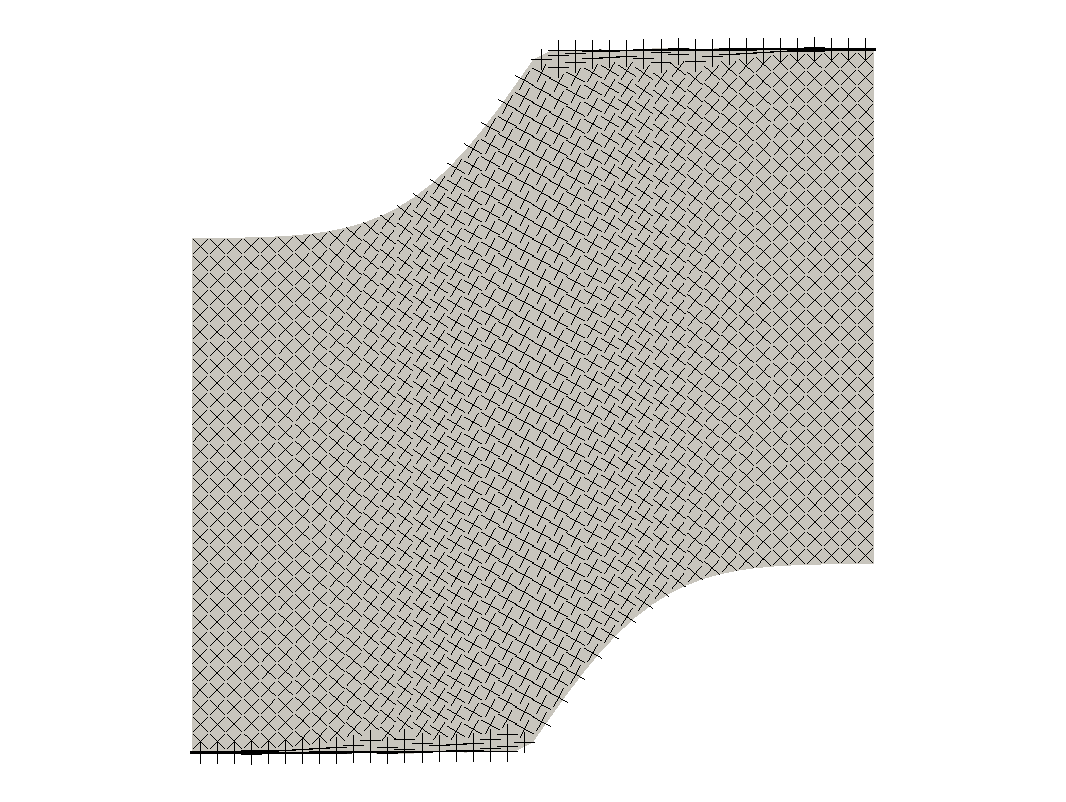
\includegraphics[width=5cm]{python_codes/fieldstone_89/results/shearband/new_dirs0005}
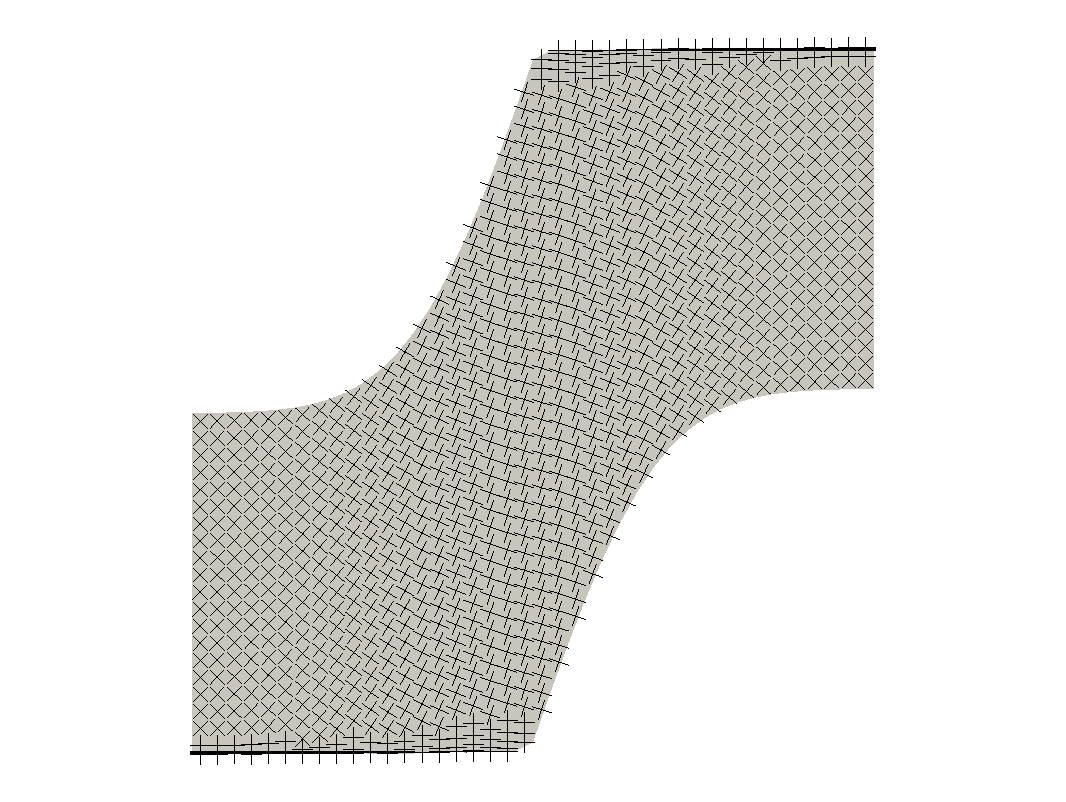
\includegraphics[width=5cm]{python_codes/fieldstone_89/results/shearband/new_dirs0010}\\
{\captionfont Directions of the principal strains. Top is old (strain rate integration), 
bottom is new (finite strain). We see that 
the old method does not record any rotation and the angles remain at 45\si{\degree}. 
The new method shows principal strains which align more and more with the direction 
of shearing towards the center.}
\end{center}


A single cell is chosen in the middle of the domain and its strain values 
recorded over time in a file:
\begin{center}
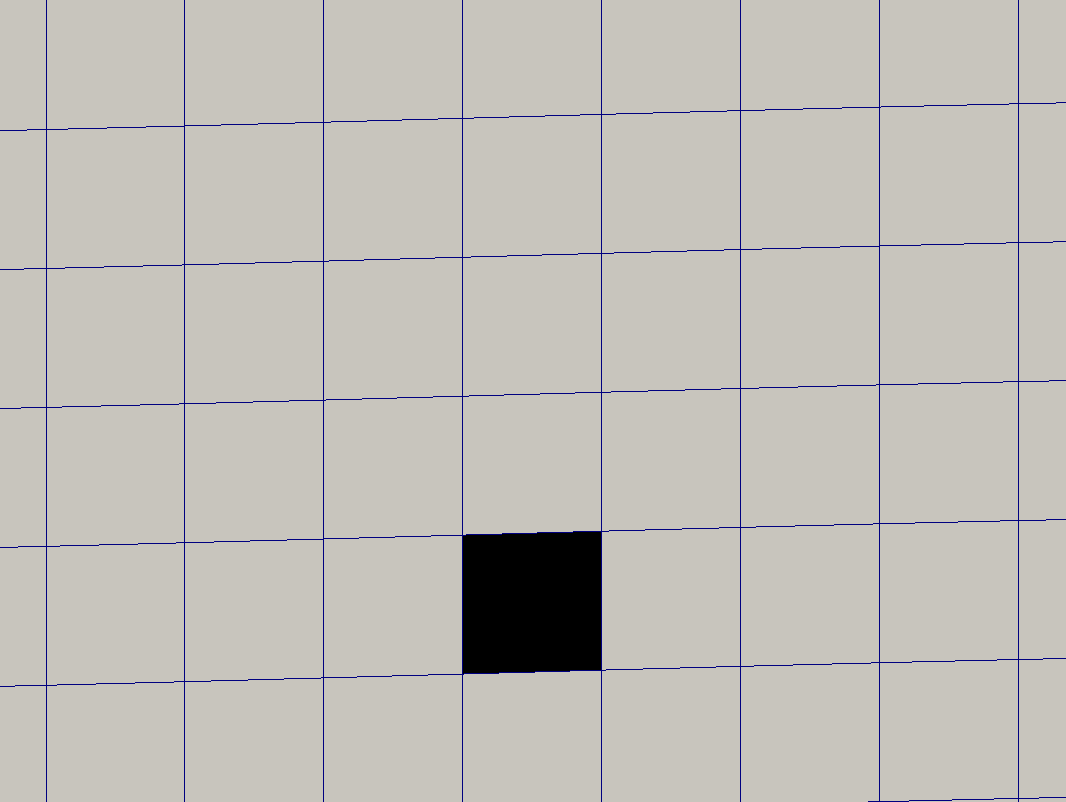
\includegraphics[width=4cm]{python_codes/fieldstone_89/results/shearband/target0000.png}
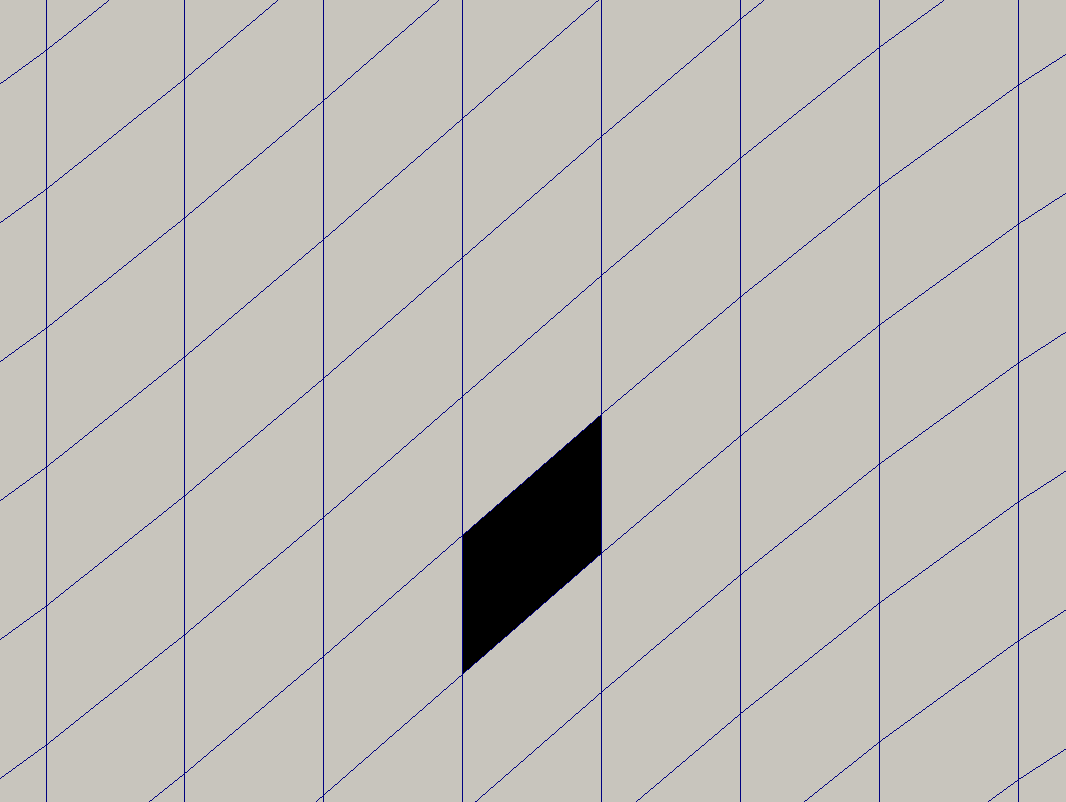
\includegraphics[width=4cm]{python_codes/fieldstone_89/results/shearband/target0003.png}
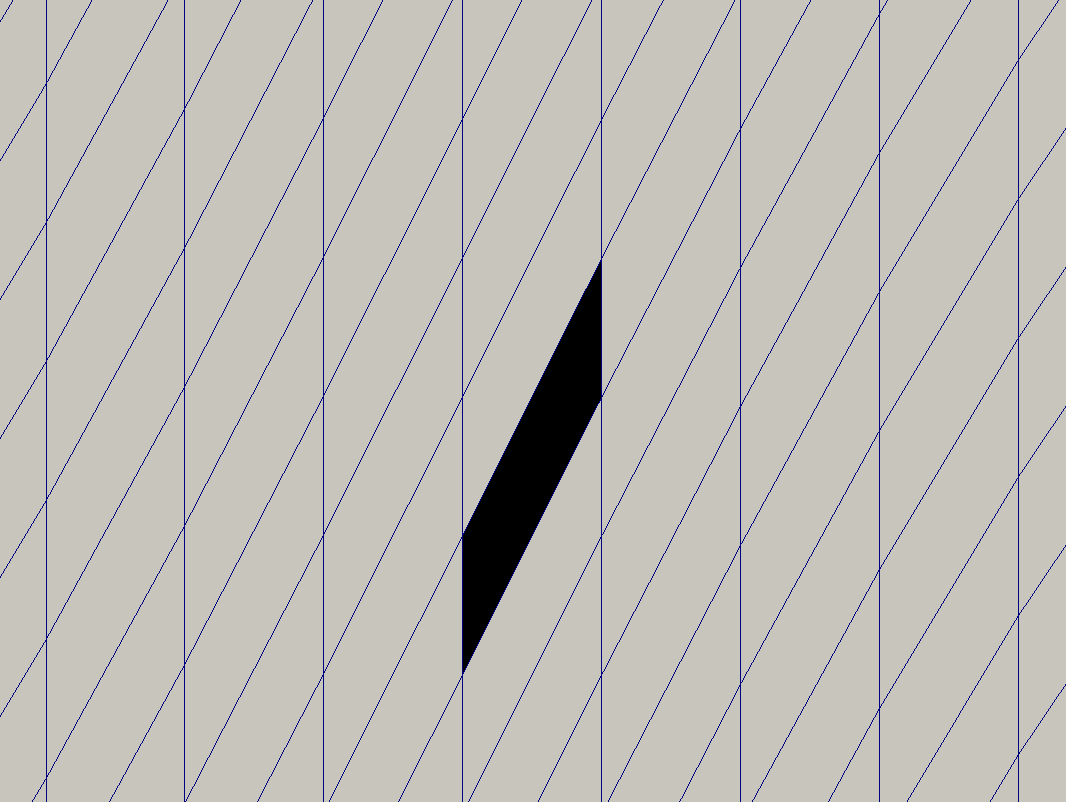
\includegraphics[width=4cm]{python_codes/fieldstone_89/results/shearband/target0007.png}
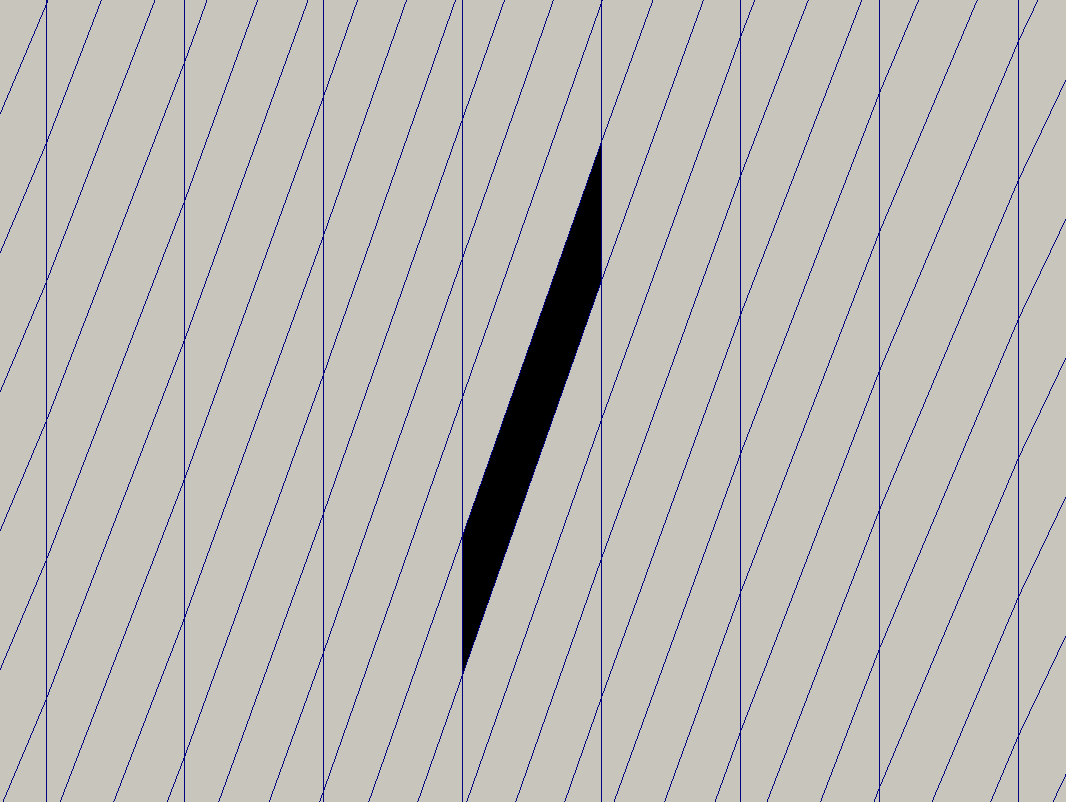
\includegraphics[width=4cm]{python_codes/fieldstone_89/results/shearband/target0010.png}\\
{\captionfont Cell undergoing deformation.}
\end{center}

\begin{center}
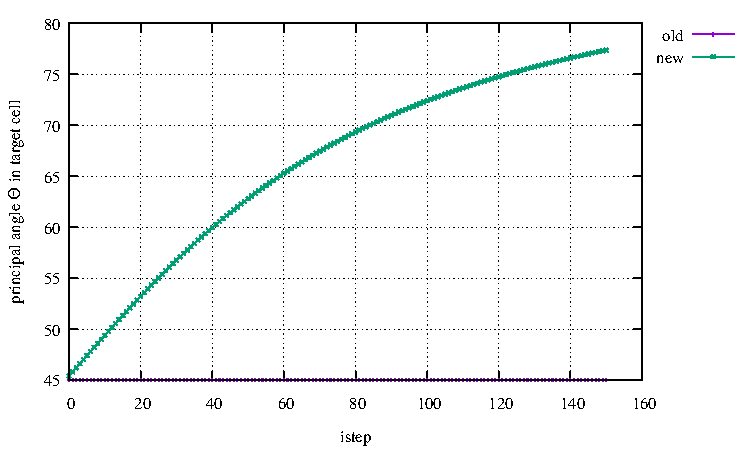
\includegraphics[width=9.cm]{python_codes/fieldstone_89/results/shearband/principal_angle.pdf}
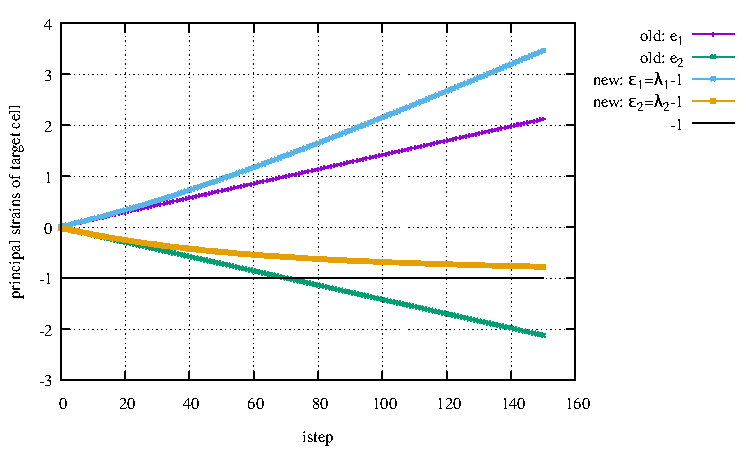
\includegraphics[width=9.cm]{python_codes/fieldstone_89/results/shearband/principal_strains.pdf}\\
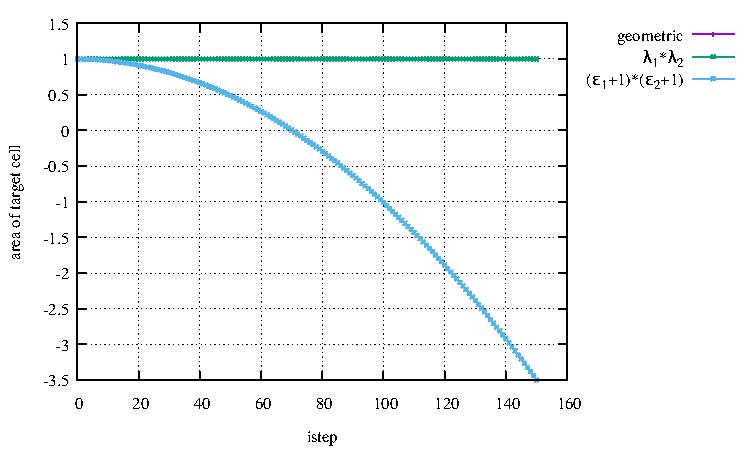
\includegraphics[width=9.cm]{python_codes/fieldstone_89/results/shearband/area.pdf}
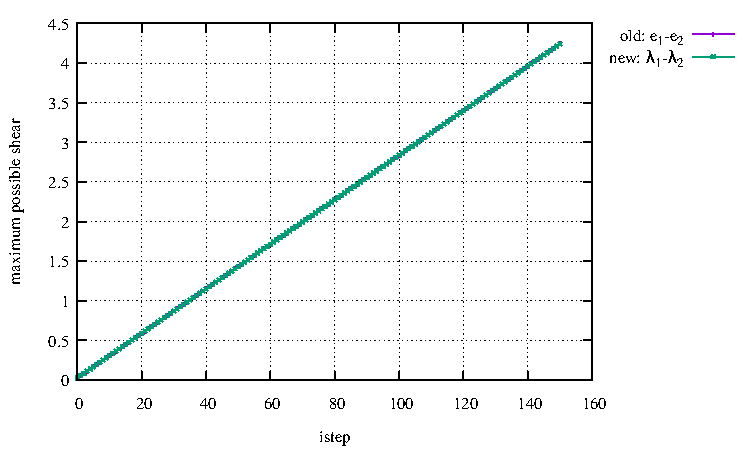
\includegraphics[width=9.cm]{python_codes/fieldstone_89/results/shearband/maximum_shear.pdf}\\
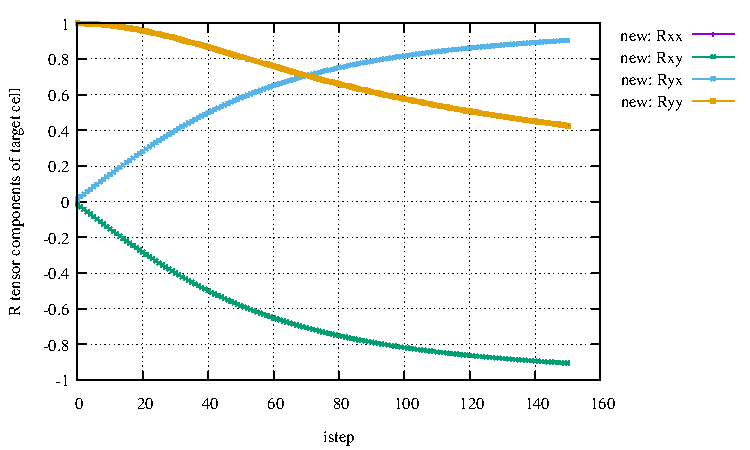
\includegraphics[width=9.cm]{python_codes/fieldstone_89/results/shearband/R.pdf}
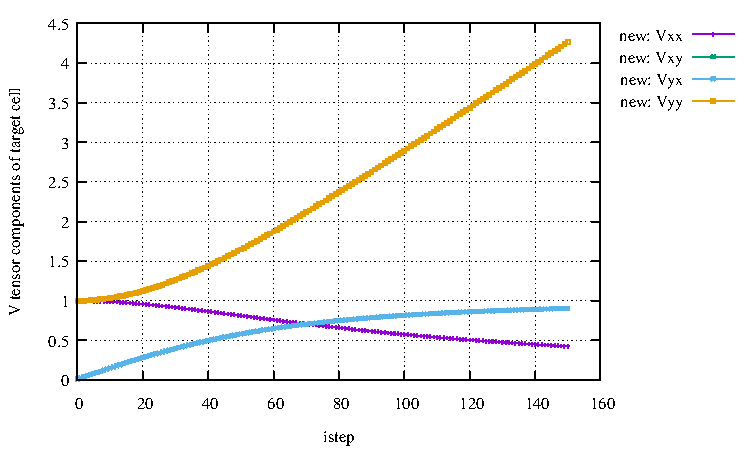
\includegraphics[width=9.cm]{python_codes/fieldstone_89/results/shearband/V.pdf}\\
{\captionfont Time evolution of the principal angle $\theta_\varepsilon$, 
the strain principal values, the relative area change of the target cell, 
the components of ${\bm R}$, the components of ${\bm V}$ and the maximum 
possible shear.}
\end{center}










\newpage
%%%%%%%%%%%%%%%%%%%%%%%%%%%%%%%%%%%%%%%%%%%%%%%%%%%%%%%%%%%%%%%%%%%%%%5
\subsection*{The vertical extension (experiment=2)} 

In this case the velocity field is prescribed to be:
\begin{eqnarray}
u(x,y)&=&0 \\
v(x,y)&=&y
\end{eqnarray}
Since the divergence of this field is not zero, volume (area) is not conserved.

The components of the strain rate tensor are
\[
\dot\varepsilon_{xx} = 0 
\qquad
\dot\varepsilon_{yy} = 1
\qquad
\dot\varepsilon_{xy} = 0 
\]
So that the components of the strain for the old method are given by:
\[
\varepsilon_{xx} = 0 
\qquad
\varepsilon_{yy} = nstep \; \delta t
\qquad
\varepsilon_{xy} = 0 
\]



\begin{center}
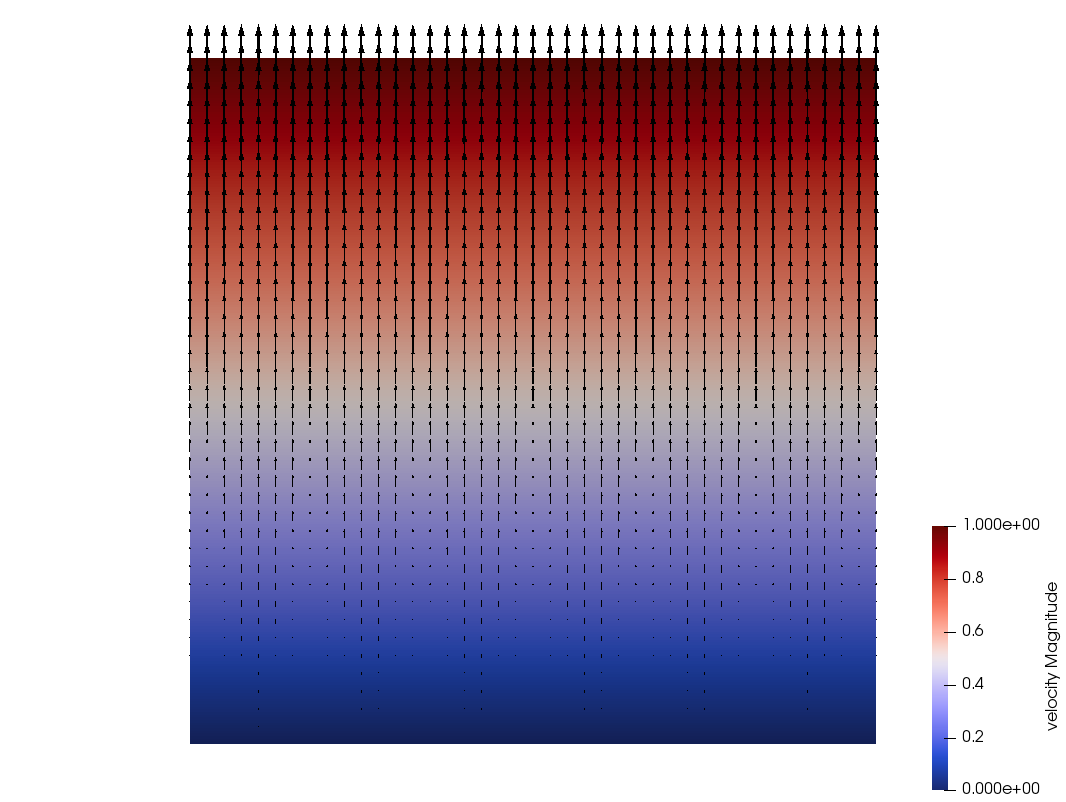
\includegraphics[width=7cm]{python_codes/fieldstone_89/results/vertical/vel}\\
{\captionfont Velocity field on Eulerian mesh}
\end{center}


\begin{center}
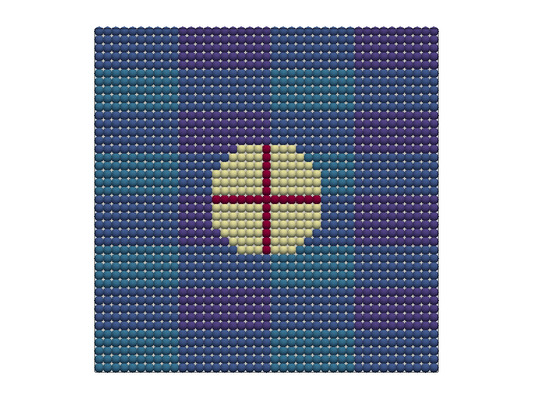
\includegraphics[width=4cm]{python_codes/fieldstone_89/results/vertical/paint0000}
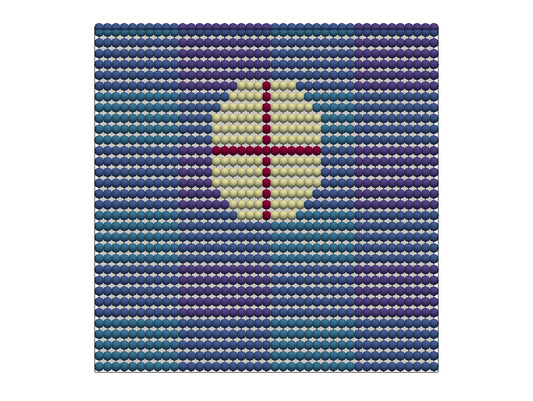
\includegraphics[width=4cm]{python_codes/fieldstone_89/results/vertical/paint0005}
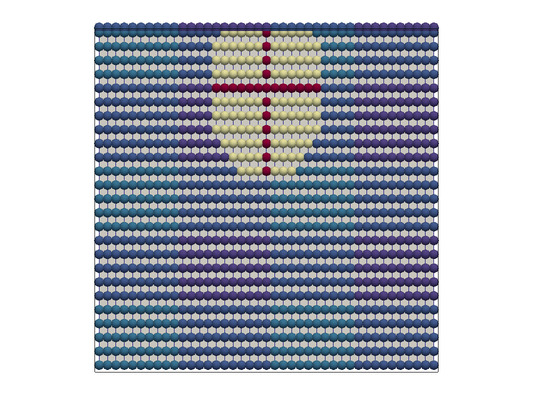
\includegraphics[width=4cm]{python_codes/fieldstone_89/results/vertical/paint0010}
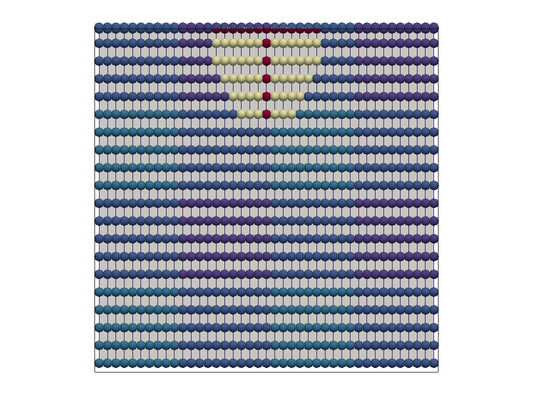
\includegraphics[width=4cm]{python_codes/fieldstone_89/results/vertical/paint0015}
\end{center}

\begin{center}
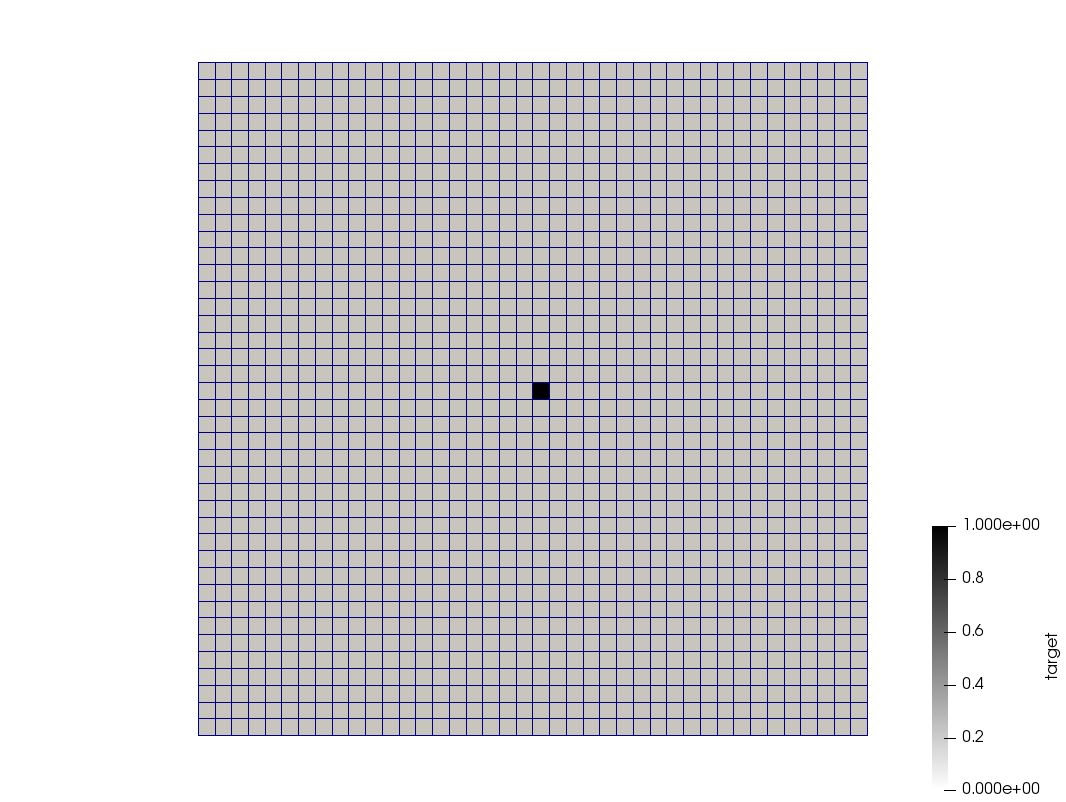
\includegraphics[width=4cm]{python_codes/fieldstone_89/results/vertical/target0000}
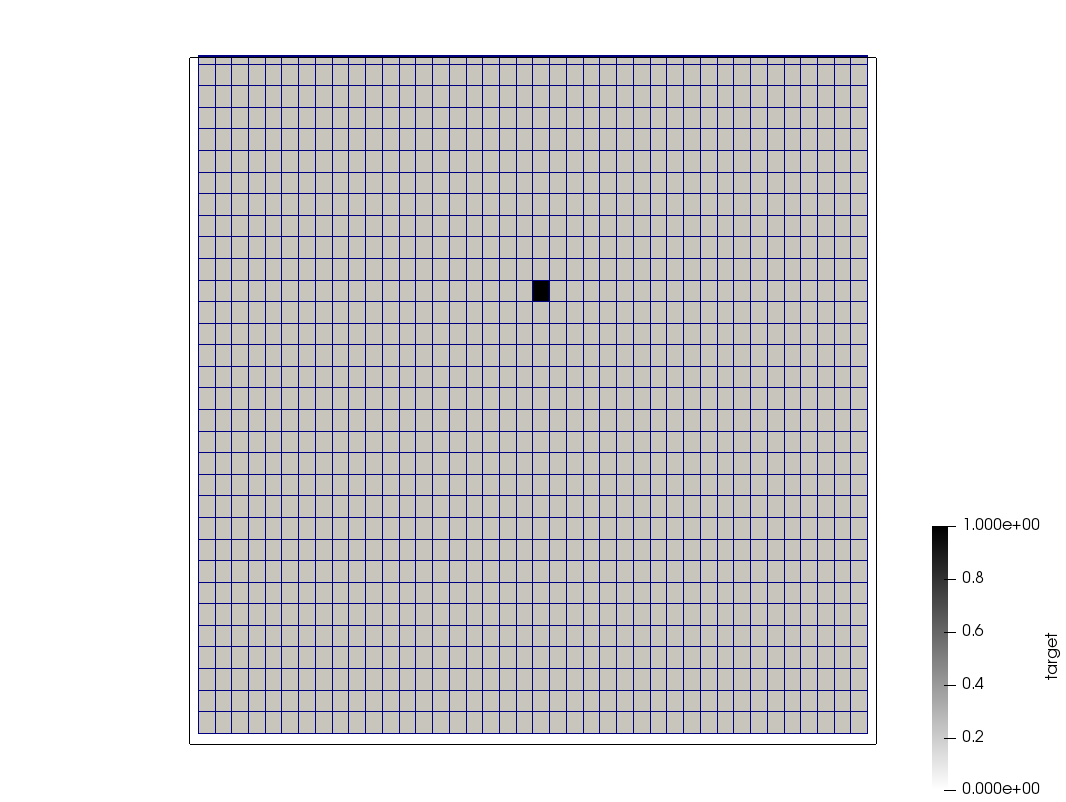
\includegraphics[width=4cm]{python_codes/fieldstone_89/results/vertical/target0005}
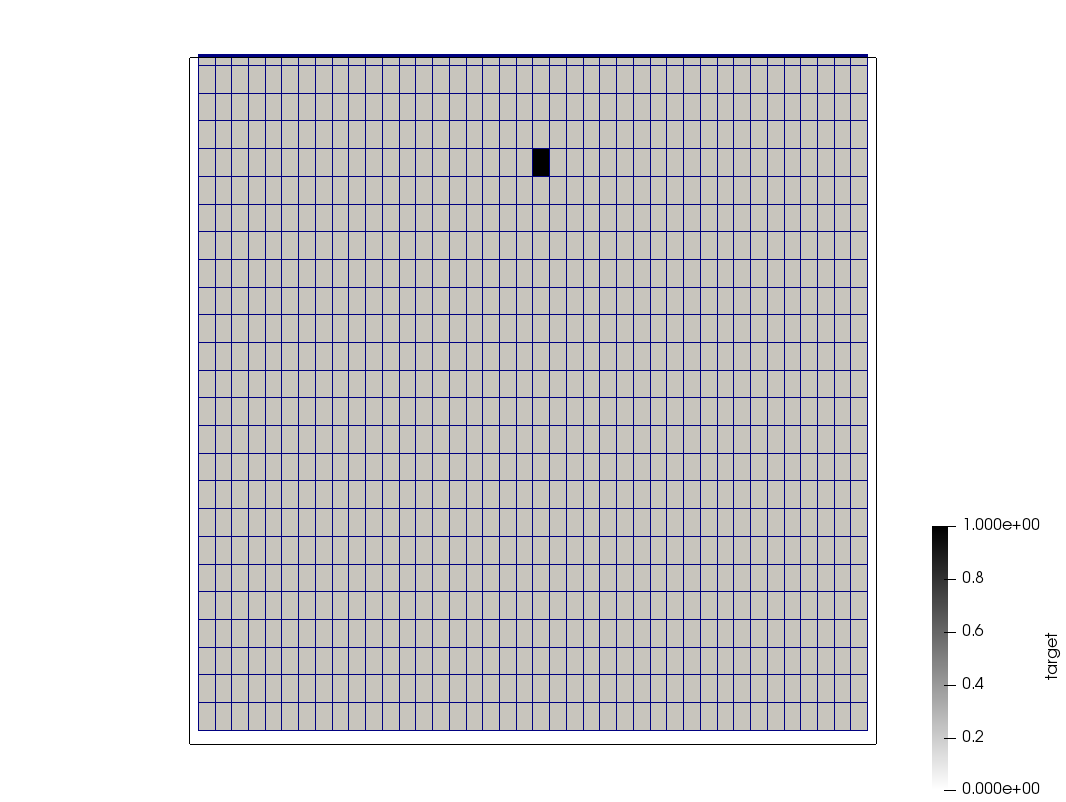
\includegraphics[width=4cm]{python_codes/fieldstone_89/results/vertical/target0010}
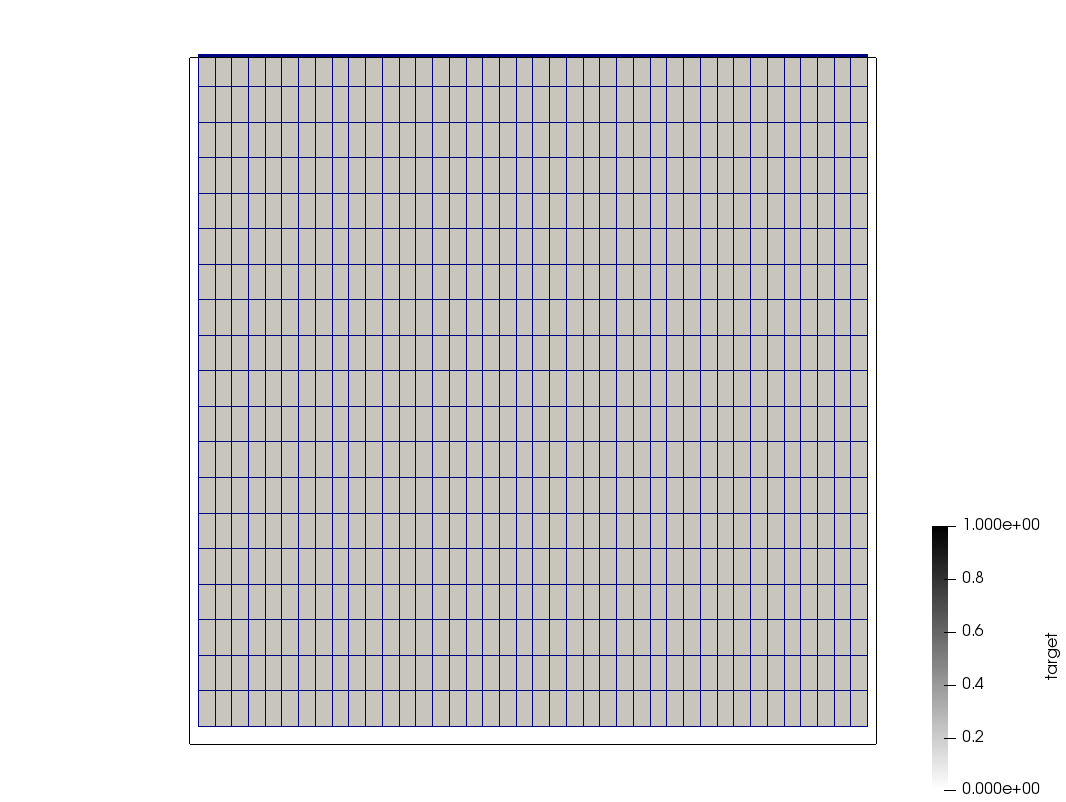
\includegraphics[width=4cm]{python_codes/fieldstone_89/results/vertical/target0015}\\
REDO
\end{center}

\begin{center}
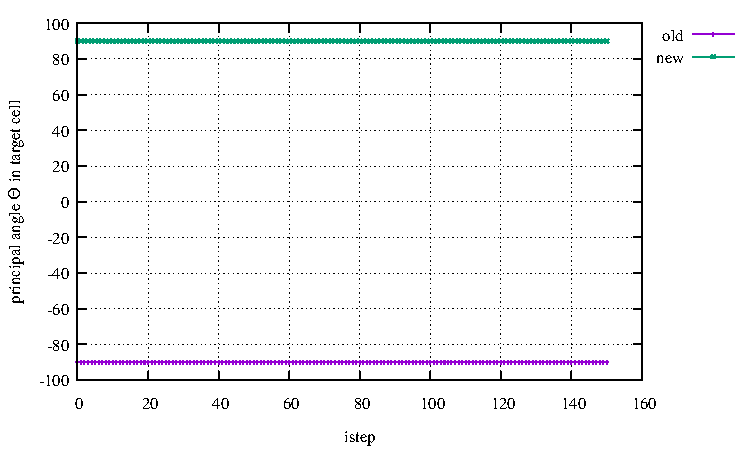
\includegraphics[width=9.5cm]{python_codes/fieldstone_89/results/vertical/principal_angle.pdf}
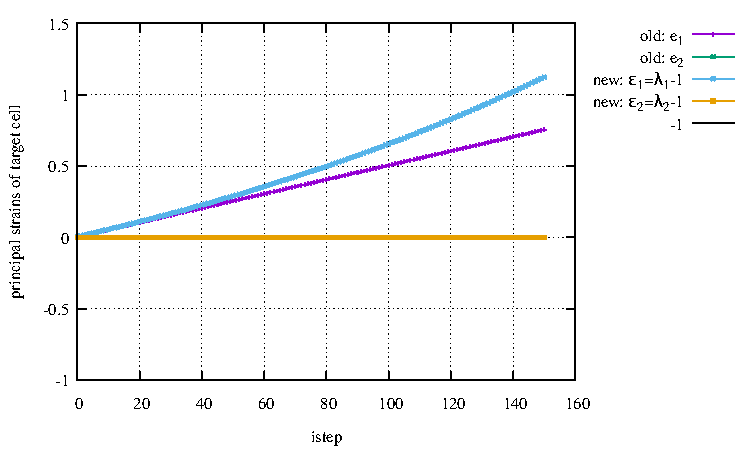
\includegraphics[width=9.5cm]{python_codes/fieldstone_89/results/vertical/principal_strains.pdf}\\
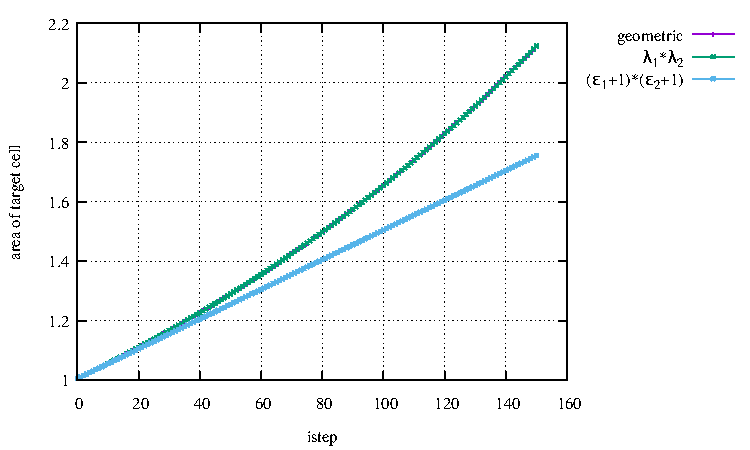
\includegraphics[width=9.5cm]{python_codes/fieldstone_89/results/vertical/area.pdf}
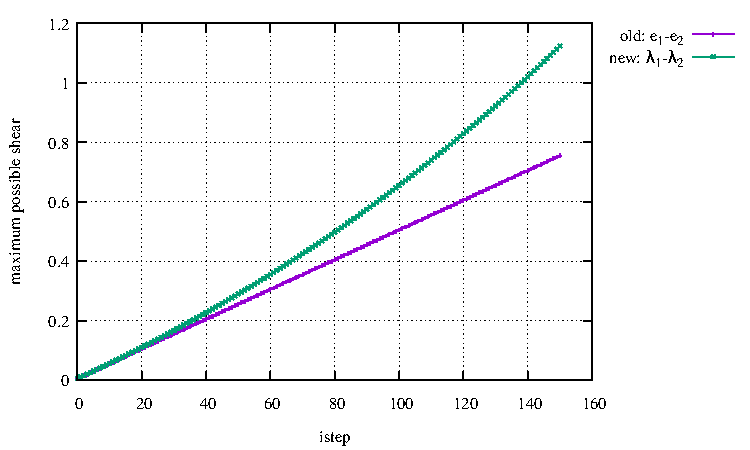
\includegraphics[width=9.5cm]{python_codes/fieldstone_89/results/vertical/maximum_shear.pdf}\\
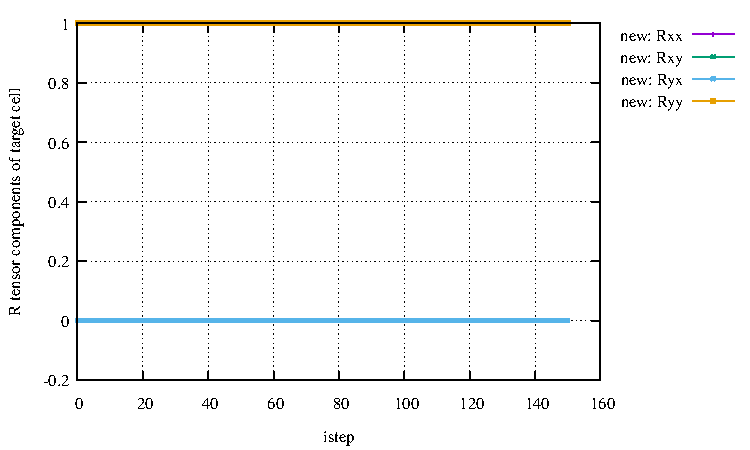
\includegraphics[width=9.5cm]{python_codes/fieldstone_89/results/vertical/R.pdf}
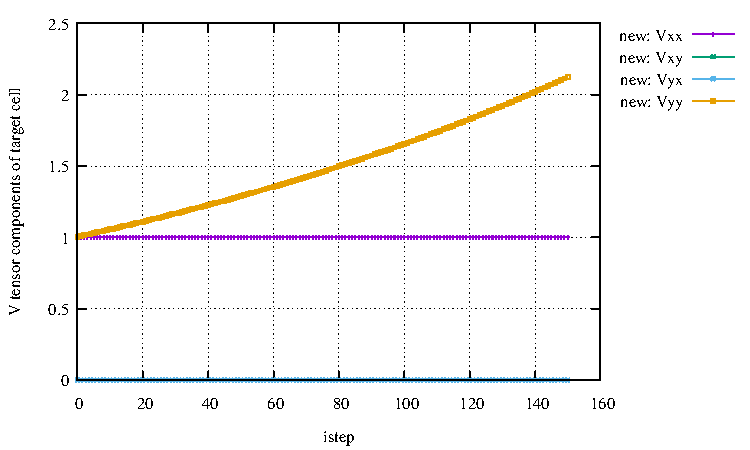
\includegraphics[width=9.5cm]{python_codes/fieldstone_89/results/vertical/V.pdf}\\
{\captionfont Time evolution of the principal angle $\theta_\varepsilon$, 
the strain principal values, the relative area change of the target cell, 
the components of ${\bm R}$, the components of ${\bm V}$ and the maximum
possible shear.}
\end{center}





\newpage
%%%%%%%%%%%%%%%%%%%%%%%%%%%%%%%%%%%%%%%%%%%%%%%%%%%%%%%%%%%%%%%%%%%%%%5
\subsection*{Pure shear (experiment=3)}

The velocity field is given by
\begin{eqnarray}
u(x,y)&=&x \nonumber\\
v(x,y)&=&y \nonumber
\end{eqnarray}
The components of the strain rate tensor are
\[
\dot\varepsilon_{xx} = 1 
\qquad
\dot\varepsilon_{yy} = 1
\qquad
\dot\varepsilon_{xy} = 0 
\]
So that the components of the strain for the old method are given by:




\begin{center}
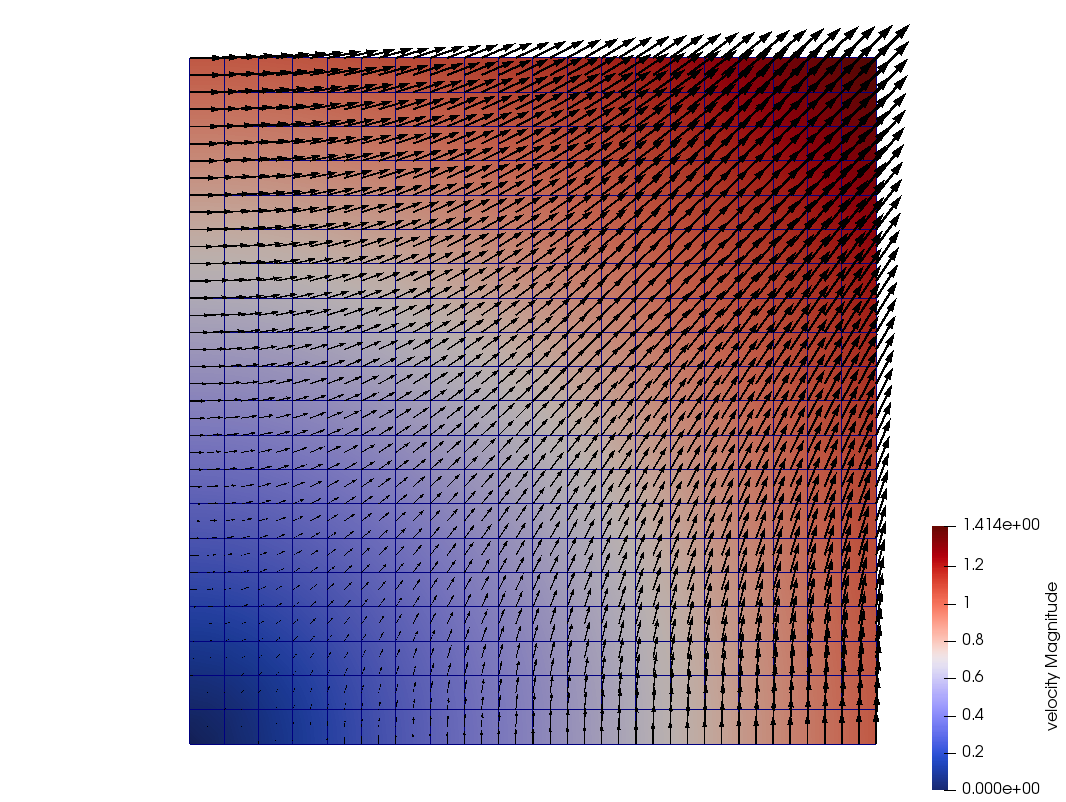
\includegraphics[width=7cm]{python_codes/fieldstone_89/results/pureshear/vel}\\
{\captionfont Velocity field on Eulerian mesh}
\end{center}

\begin{center}
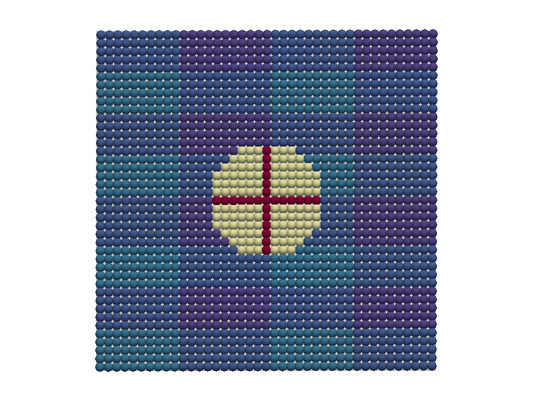
\includegraphics[width=4cm]{python_codes/fieldstone_89/results/pureshear/paint0000}
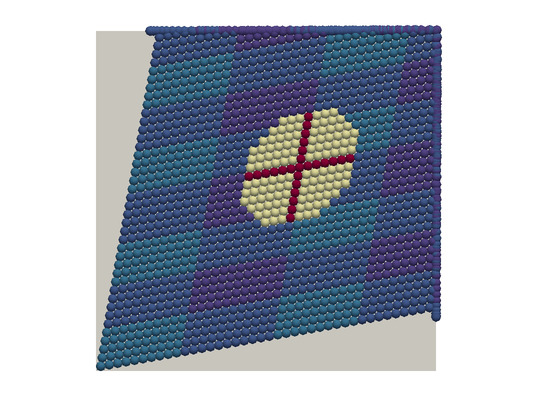
\includegraphics[width=4cm]{python_codes/fieldstone_89/results/pureshear/paint0005}
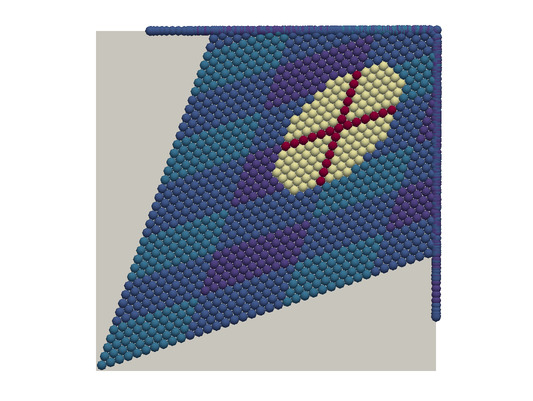
\includegraphics[width=4cm]{python_codes/fieldstone_89/results/pureshear/paint0010}\\
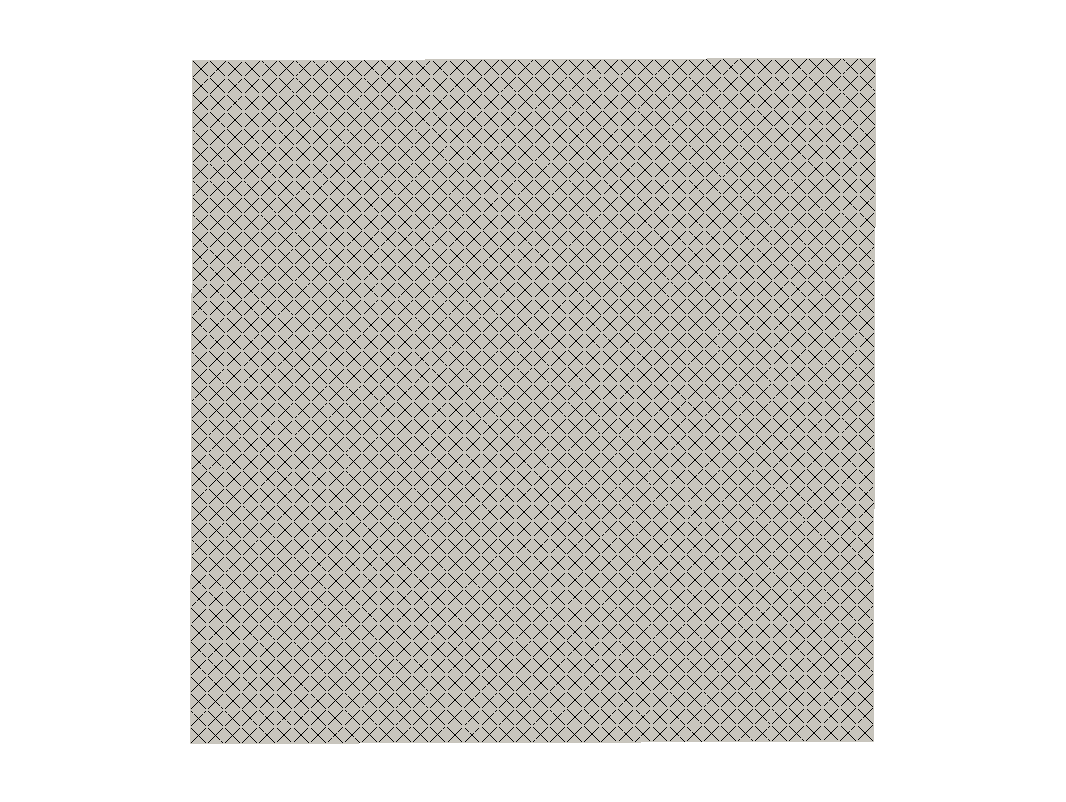
\includegraphics[width=4cm]{python_codes/fieldstone_89/results/pureshear/old_dirs0000}
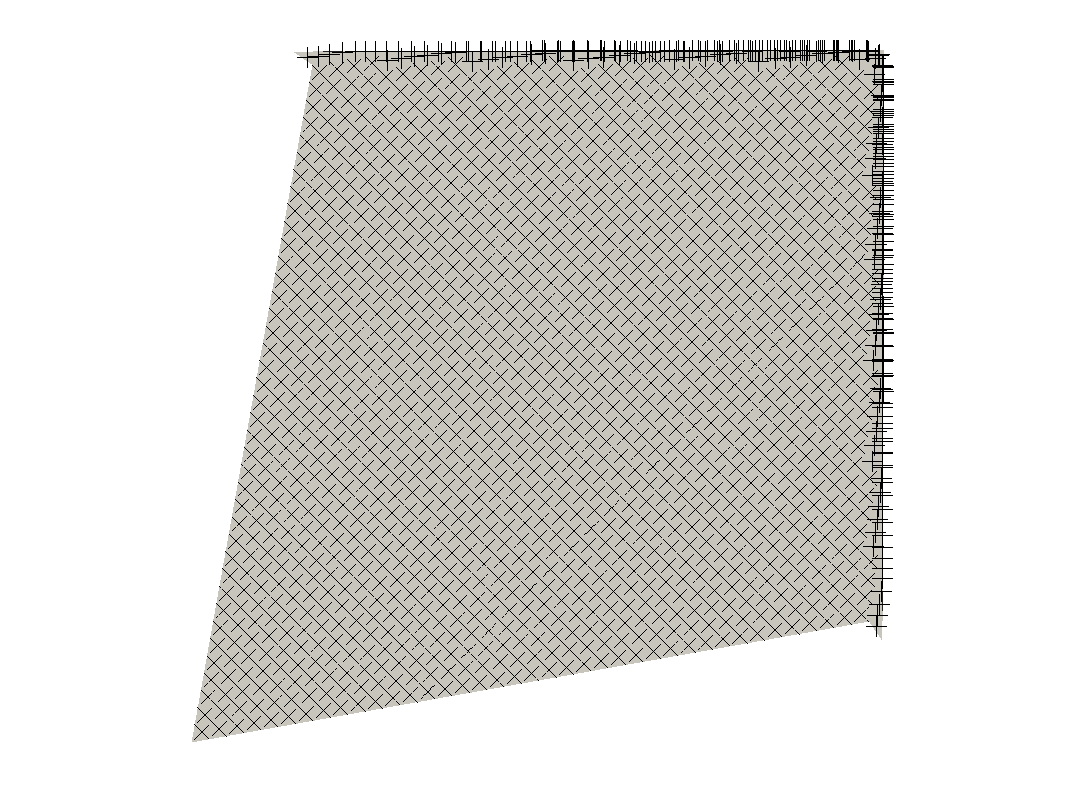
\includegraphics[width=4cm]{python_codes/fieldstone_89/results/pureshear/old_dirs0005}
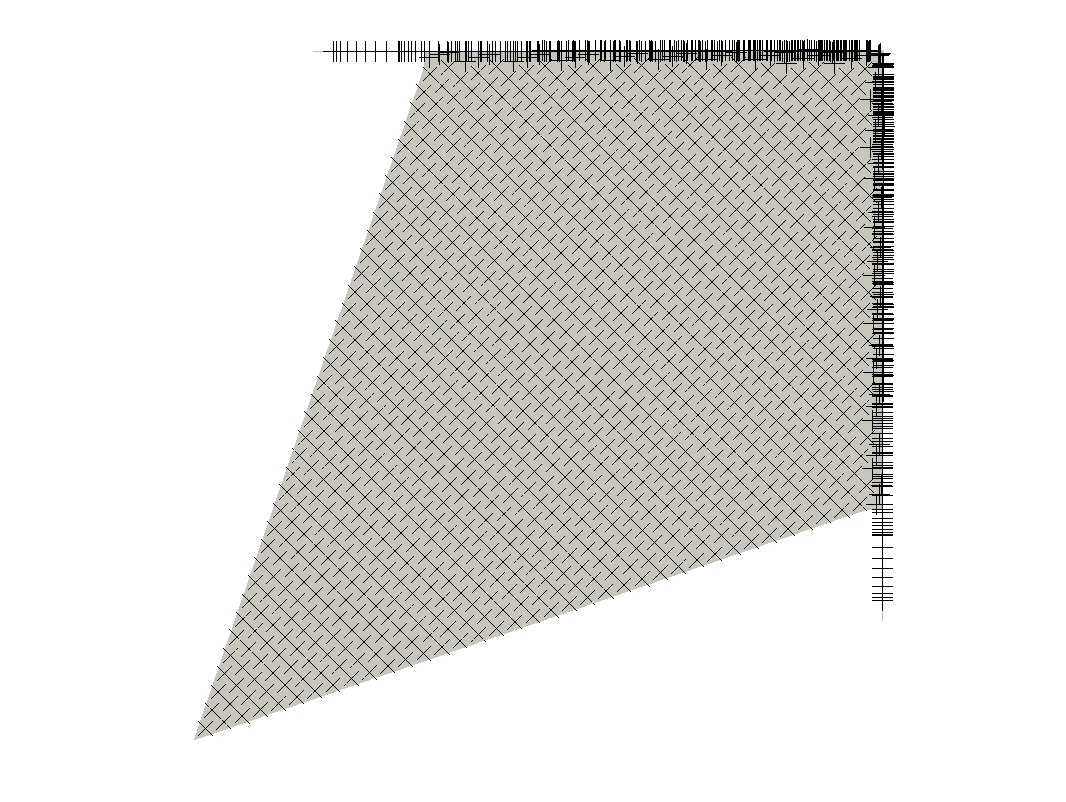
\includegraphics[width=4cm]{python_codes/fieldstone_89/results/pureshear/old_dirs0010}\\
{\captionfont old and new are identical}
\end{center}

\begin{center}
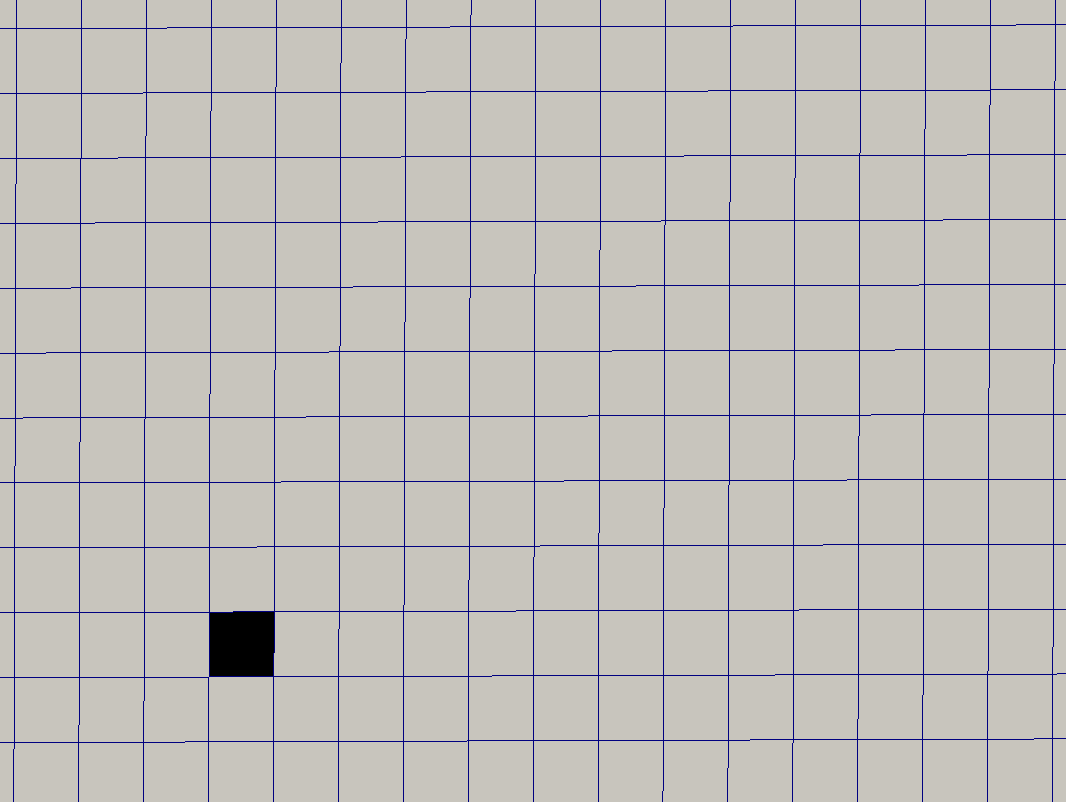
\includegraphics[width=3cm]{python_codes/fieldstone_89/results/pureshear/target0000}
\includegraphics[width=3cm]{python_codes/fieldstone_89/results/pureshear/target0005}
\includegraphics[width=3cm]{python_codes/fieldstone_89/results/pureshear/target0010}
\end{center}


\begin{center}
\includegraphics[width=9.5cm]{python_codes/fieldstone_89/results/pureshear/principal_angle.pdf}
\includegraphics[width=9.5cm]{python_codes/fieldstone_89/results/pureshear/principal_strains.pdf}\\
\includegraphics[width=9.5cm]{python_codes/fieldstone_89/results/pureshear/area.pdf}
\includegraphics[width=9.5cm]{python_codes/fieldstone_89/results/pureshear/maximum_shear.pdf}\\
\includegraphics[width=9.5cm]{python_codes/fieldstone_89/results/pureshear/R.pdf}
\includegraphics[width=9.5cm]{python_codes/fieldstone_89/results/pureshear/V.pdf}\\
{\captionfont Time evolution of the principal angle $\theta_\varepsilon$, 
the strain principal values, the relative area change of the target cell, 
the components of ${\bm R}$, the components of ${\bm V}$ and the maximum
possible shear.}
\end{center}

\newpage
%%%%%%%%%%%%%%%%%%%%%%%%%%%%%%%%%%%%%%%%%%%%%%%%%%%%%%%%%%%%%%%%%%%%%%5
\subsection*{Bi-axial stretch (experiment=4)}

The velocity is given by
\begin{eqnarray}
u(x,y)&=&-x+L_x/2 \\
v(x,y)&=&y-L_y/2
\end{eqnarray}
The components of the strain rate tensor are
\[
\dot\varepsilon_{xx} = -1 
\qquad
\dot\varepsilon_{yy} = 1
\qquad
\dot\varepsilon_{xy} = 0 
\]
The velocity divergence is zero. The components of the strain for the old method are given by:




\begin{center}
\includegraphics[width=7cm]{python_codes/fieldstone_89/results/biaxial/vel}\\
{\captionfont Velocity field on Eulerian mesh}
\end{center}


\begin{center}
\includegraphics[width=4cm]{python_codes/fieldstone_89/results/biaxial/target0000}
\includegraphics[width=4cm]{python_codes/fieldstone_89/results/biaxial/target0005}
\includegraphics[width=4cm]{python_codes/fieldstone_89/results/biaxial/target0010}
\end{center}

\begin{center}
\includegraphics[width=4cm]{python_codes/fieldstone_89/results/biaxial/paint0000}
\includegraphics[width=4cm]{python_codes/fieldstone_89/results/biaxial/paint0005}
\includegraphics[width=4cm]{python_codes/fieldstone_89/results/biaxial/paint0010}
\includegraphics[width=4cm]{python_codes/fieldstone_89/results/biaxial/paint0015}
\end{center}

\begin{center}
\includegraphics[width=4cm]{python_codes/fieldstone_89/results/biaxial/new_dirs0000}
\includegraphics[width=4cm]{python_codes/fieldstone_89/results/biaxial/new_dirs0005}
\includegraphics[width=4cm]{python_codes/fieldstone_89/results/biaxial/new_dirs0010}
\includegraphics[width=4cm]{python_codes/fieldstone_89/results/biaxial/new_dirs0015}
\end{center}

\begin{center}
\includegraphics[width=9.cm]{python_codes/fieldstone_89/results/biaxial/principal_angle.pdf}
\includegraphics[width=9.cm]{python_codes/fieldstone_89/results/biaxial/principal_strains.pdf}\\
\includegraphics[width=9.cm]{python_codes/fieldstone_89/results/biaxial/area.pdf}
\includegraphics[width=9.cm]{python_codes/fieldstone_89/results/biaxial/maximum_shear.pdf}\\
\includegraphics[width=9.cm]{python_codes/fieldstone_89/results/biaxial/R.pdf}
\includegraphics[width=9.cm]{python_codes/fieldstone_89/results/biaxial/V.pdf}\\
{\captionfont Time evolution of the principal angle $\theta_\varepsilon$, 
the strain principal values and the area of the target cell.}
\end{center}

PB: e2 cannot become less than -1 


\subsection*{Discussion 'old' vs. 'new' cumulative strain}

The first observation is that all quantities from the 'old' (integrated strain rates) and 'new' 
(strain computed from cumulative displacements) start at the same values. 
The 'old' cumulative strains are thus an acceptable approximation for small deformations. 
For increasing deformation a number of problems arise with the 'old' strains:

\begin{itemize}
\item principal axes do not rotate for simple shear (The shear band, experiment 1) while they should continuously change
\item principal strain values deviate from the exact values (the 'new' principal strains) (all experiments)
\item negative principal strains for the 'old' definition can decrease below the theoretical limit of -1 (The shear band, experiment 1; bi-axial stretch, experiment 4)
\item related to the previous point, the area computed from these principal strains may incorrectly become negative (The shear band, experiment 1;  bi-axial stretch, experiment 4)
\item the maximum shear deviates from the correct value (all experiments except for experiment 1)
\end{itemize}

The problems in the integration of strain rates is due to two causes. Firstly, strain rates are determined relative to the current state (already deformed), which means that the state with respect the deformation is defined changes during integration. Rather, the 'new' strains based on the cumulative  displacements are all references with respect to the original, undeformed, configuration. Secondly, because incremental principal axes change during general deformation that contains simple shear or rigid body rotation (which does not occur for the special cases of experiment 2, 3 and 4), incremental strains cannot be summed \cite{malvern}. In the special cases where there is no rotation, strain rates may be integrated, and the result is a strain measure called natural strain or Hencky strain \cite{malvern}.


\Literature: McKenzie (1979) \cite{mcke79} , McKenzie \& Jackson (1983) \cite{mcja83}

